% !Mode:: "TeX:UTF-8"
%!TEX program  = xelatex
%\PassOptionsToPackage{draft}{graphicx}
\documentclass[bwprint,fontset=fandol]{gmcmthesis}

\hypersetup{hidelinks}

%========================================================
% 题目、摘要、关键词标题：隶书，小二
% 字体文件位置：Fonts/SIMLI.TTF
%========================================================

% 定义真正的隶书字体
\setCJKfamilyfont{mylishu}[
    Path = Fonts/
]{SIMLI.TTF}

% 将模板中的 \lishu 指向上传的真正隶书
\renewcommand{\lishu}{\CJKfamily{mylishu}}

%========================================================
% 将“关键词”三个字统一修改为：隶书、小二
%========================================================
\makeatletter

\renewcommand{\keywords}[1]{%
    \renewcommand{\gmcm@tokens@keywords}{#1}%
    \par
    \vskip1ex
    {\noindent\zihao{-2}\lishu
    \gmcm@cap@keywordsname：}%
    ~{\gmcm@tokens@keywords}%
}

\makeatother
% \usepackage{graphicx}   % 必须，否则 \includegraphics 报错

% Support for the added equations, editable tables and figure placeholders.
\usepackage{amsmath,amssymb}
\usepackage{array,booktabs,tabularx,longtable}
\usepackage{float,placeins}

%\usepackage[framemethod=TikZ]{mdframed}

%\usepackage{fontspec}  % for Consolas & Courier New
%\lstset{basicstyle=\small\fontspec{Consolas}}
%\lstset{basicstyle=\small\fontspec{Courier New}}
%\setmonofont{Consolas}
%\setcounter{tocdepth}{3}   % 调整目录深度
\usepackage{siunitx}
\usepackage{colortbl}
\definecolor{color1}{rgb}{0.78,0.88,0.99}
\definecolor{color2}{rgb}{0.36,0.62,0.84}
%\definecolor{color3}{rgb}{0.8235,0.8706,0.9373}
\definecolor{color3}{rgb}{0.88,0.92,0.96}
\definecolor{color4}{rgb}{0.96,0.97,0.98}%{0.9176,0.9373,0.9686}

% 算法
\usepackage[noend]{algpseudocode}
\usepackage{algorithmicx,algorithm}
\floatname{algorithm}{算法}
\renewcommand{\algorithmicrequire}{\textbf{输入:}}
\renewcommand{\algorithmicensure}{\textbf{输出:}}

%\numberwithin{equation}{section}
%\numberwithin{figure}{section}
%\numberwithin{table}{section}


\newcommand{\red}[1]{\textcolor{red}{#1}}
\newcommand{\blue}[1]{\textcolor{blue}{#1}}


%===================== 建模论文题目 ======================

\title{山区洪涝灾害下无人机运输与通信协同优化
}
\baominghao{\hspace{6em} 26106350114} %参赛队号
\schoolname{\hspace{5.8em} 西南大学} %学校名称
\membera{\hspace{6em} 谢文哲} %队员A
\memberb{\hspace{6em} 章林怡} %队员B
\memberc{\hspace{6em} 刘宇豪} %队员C

%=======================================================


\begin{document}

%生成标题
\maketitle

%填写摘要
\begin{abstract}

山区洪涝灾害往往伴随着\textbf{道路阻断、通信受损与能源受限}等多重约束，使传统地面运输难以及时完成应急物资配送。无人机具有机动性强、受地面道路影响小等优势，但其实际救援能力同时受到载荷、地形、能耗、配送时限、通信覆盖以及设备周转等因素制约。针对山区洪涝灾害场景下无人机应急运输与通信保障的协同优化问题，本文结合服务区空间位置、数字高程模型（DEM）、货箱需求、异构无人机参数、电池资源及无线通信链路参数，建立了由\textbf{单点运输能力分析、多机多架次调度、运输--通信联合调度和任务分区资源配置}构成的递进式优化模型，并从运输效率、任务及时性、能源消耗和资源占用等多个维度对方案进行评价。

针对问题一，为准确刻画不同机型在山区地形条件下的运输能力，首先利用\textbf{DEM栅格采样}提取调度中心与各服务区直线路径上的最高地形高程，并按照“爬升--巡航--下降”的飞行过程建立时间与能耗计算模型。在载荷影响等效航程且返航需保留安全能量余量的条件下，利用\textbf{二分搜索}求解各“机型--服务区”组合的最大安全载荷。在此基础上，将不可拆货箱的组批过程转化为同时考虑载质量、装载体积与安全能量约束的\textbf{多维装箱优化问题}，以架次数、总运输能耗和累计作业时间构造分层多目标优化模型，获得各服务区的货箱组批与机型选择方案。同时改变返航安全余量进行敏感性分析，刻画安全冗余增加对最大可运输载荷及架次数的影响规律。

针对问题二，在单架次可访问多个服务区的条件下，进一步考虑\textbf{异构无人机、共享电池、配送时限与多架次周转}之间的耦合关系。本文构建带容量、能量和时间窗约束的异构多旅行车辆路径模型，将货箱组批、服务区访问顺序、运输机型、实体无人机、电池资源及架次开始时刻进行联合决策。为降低大规模组合搜索的复杂度，采用\textbf{“可行架次生成--资源调度优化”两阶段求解框架}：首先生成满足载荷、体积和能量限制的候选运输架次，再结合医疗物资期望送达时间和首批保障截止时间，通过自适应邻域搜索与整数优化对路线及资源时序进行协调。模型能够输出逐架次运输路线、逐箱送达时刻以及无人机和电池占用情况，并通过任务时序和资源冲突检验保证方案的实际可执行性。

针对问题三，在运输调度基础上进一步引入山区地形遮挡和无线传播约束。首先依据运输无人机的连续飞行轨迹，结合DEM完成\textbf{视距（LOS）遮挡判定}，并根据双向链路预算计算运输无人机与固定网关之间的实时通信可用性。对于直连链路失效区段，在DEM覆盖区域内生成满足悬停高度约束的候选中继位置，并预计算“运输无人机--中继无人机--固定网关”两段链路的可服务关系，从而将连续空间中继部署问题转化为有限候选位置上的\textbf{时空覆盖问题}。进一步建立运输无人机与中继无人机联合调度模型，同时优化运输架次、中继悬停位置、服务时段及能源组件配置，在保证运输无人机\textbf{全飞行过程连续通信}的前提下，综合降低物资延误、联合任务完成时间、运输与中继总能耗以及设备使用强度，并通过时间离散精度的敏感性分析验证通信判定结果的稳定性。

针对问题四，为研究灾后分区独立救援条件下的资源配置问题，根据问题三中已经确定的运输架次和通信保障关系构建\textbf{服务区任务耦合图}。若多个服务区位于同一运输架次或存在不可分割的联合保障关系，则将其合并为不可拆分的任务单元，并分别建立两分区和三分区优化模型。在保持原运输与中继任务安排不变的条件下，以\textbf{资源配置规模、资源冗余、组间工作量均衡和现有库存缺口}为主要评价指标进行分区优化；同时基于任务占用时间区间计算各分区运输无人机、共享电池、中继无人机及能源组件的最大并发需求，从而得到各分区独立执行所需的最小资源配置，并识别潜在资源瓶颈及其形成原因。

综上，本文将\textbf{地形约束、运输调度、能源周转与连续通信保障}统一纳入山区应急无人机救援决策框架，在保证货箱不可拆分、任务时限、返航安全以及通信连续性的基础上，实现了由单架次能力分析到多机协同、再到运输--通信联合优化与灾区资源分区配置的逐层扩展。所建立模型具有明确的物理含义和较好的可解释性，可为山区洪涝灾害条件下无人机应急运输与通信资源协同配置提供定量化决策依据。

\keywords{山区洪涝灾害\quad  无人机应急运输\quad 异构多架次调度\quad  通信中继  \quad  协同优化}
\end{abstract}

\pagestyle{plain}

%目录 不推荐加
\maketoc

\clearpage

\section{问题重述}

\subsection{引言}   % 问题的背景
山区洪涝灾害具有突发性强、地形复杂和基础设施易受损等特点。持续强降雨可能引发山洪、滑坡及道路塌方，并进一步造成道路、供电和通信设施同时中断，使部分受灾区域在短时间内难以通过传统地面交通获得物资补给。题目所描述的广西横州市镇龙乡洪涝灾害中，就曾出现断路、断电、断网以及大量群众受困的情况，食品、饮用水、药品及抢修设备需要依靠徒步或空中方式运入灾区。 因此，利用受地面道路条件影响较小的无人机开展应急物资运输，对提高山区灾害救援效率具有重要意义。

然而，山区无人机救援并非简单的物资配送问题。一方面，复杂地形会影响无人机的飞行高度、航程及能源消耗，不同货箱的重量、体积和配送时限也使货箱组批、路径规划、机型选择和电池周转相互制约；另一方面，山体遮挡可能导致运输无人机与固定网关之间通信中断，需要利用中继无人机提供持续通信保障。由此，运输任务、通信保障和有限装备资源之间形成了明显的耦合关系。题目也明确要求同时考虑载荷、地形净空、能源储备、任务时限及通信链路等多种因素。

基于此，本文以题目给出的调度中心、15个服务区、80个不可拆货箱以及运输无人机、中继无人机、共享电池和DEM等数据为基础，围绕单点运输能力、多机多架次调度、运输与通信协同以及任务分区资源配置四个层次展开建模，在保证运输安全、配送时效和通信连续性的前提下，对有限无人机及能源资源进行合理配置，为山区洪涝灾害下的无人机应急救援提供定量化决策依据。
\subsection{问题的提出}

%\subsubsection{问题的提出内容一}

\noindent 根据题目给定的调度中心、服务区、货箱需求、DEM地形数据、运输与中继无人机参数、电池资源及通信链路参数，需要依次解决以下四个相互递进的问题。

\textbf{问题一：} 单点往返运输能力与货箱组批。针对不同机型在各服务区执行
$O_{01}\rightarrow S_i\rightarrow O_{01}$
往返任务的场景，结合DEM地形、载荷和能耗约束，确定各机型的\textbf{最大安全载荷}。在货箱不可拆分的条件下，优化\textbf{货箱组批方案}，并分析返航安全余量变化对运输能力和组批结果的影响。

\textbf{问题二：} 异构无人机多点多架次运输调度。在允许单架次访问多个服务区的条件下，综合考虑载荷、配送时限、无人机数量及共享电池周转等约束，联合优化\textbf{货箱组批、访问顺序、无人机分配和架次时序}，以提高配送及时性并降低任务完成时间、能耗和架次数。

\textbf{问题三：} 通信约束下的运输与中继联合调度。在问题二的基础上引入山区地形遮挡和通信链路约束，当运输无人机与固定网关 $G_{01}$ 无法直连时，通过中继无人机提供通信保障。联合优化\textbf{运输任务与中继无人机的悬停位置、服务时段及能源配置}，保证运输全过程通信连续，并兼顾时效与能耗。

\textbf{问题四：} 救援任务分区与资源配置。在保持问题三运输与通信任务关系不变的条件下，将 $15$ 个服务区分别划分为 $2$ 个和 $3$ 个任务组。比较不同分区方案下的\textbf{资源需求、资源冗余、工作量均衡及库存缺口}，确定更合理的分区与资源配置方案。

\clearpage

\section{模型假设与符号说明}
\subsection{模型假设}
\subsection{符号说明}
\begin{table}[htp!]
\centering
\renewcommand\arraystretch{1.2} %定义表格高度
\newcolumntype{L}{>{\quad}X}
\newcolumntype{P}[1]{>{\centering\arraybackslash}p{#1}}
\newcolumntype{C}{>{\centering \arraybackslash}X}
\newcolumntype{R}{>{\raggedright \arraybackslash}X}
\begin{tabularx}{0.9\textwidth}{|P{1.8cm}|L|}
  \hline %\toprule
  符号    &   \quad 意义 \\
  \hline %\midrule
  $ O_{01} $  &  临时调度中心    \\
  \hline
  $ G_{01} $  &  固定通信网关    \\
  \hline
  $ S_i $  &  第 $ i $ 个服务区，$ i=1,2,\ldots,15 $    \\
  \hline
  $ g $  &  运输无人机机型，$ g \in \{A,B,C\} $    \\
  \hline
  $ m_g $  &  机型 $ g $ 的无人机空机质量/kg    \\
  \hline
  $ Q_g $  &  机型 $ g $ 的额定最大载货质量/kg    \\
  \hline
  $ V_g $  &  机型 $ g $ 的最大装载体积/m$^3$    \\
  \hline
  $ E_g $  &  机型 $ g $ 单组电池可用能量/kWh    \\
  \hline
  $ p_g $  &  机型 $ g $ 的返航安全余量比例    \\
  \hline
  $ v_g $  &  机型 $ g $ 的水平巡航速度/(m·s$^{-1}$)    \\
  \hline
  $ v_g^\uparrow, v_g^\downarrow $  &  机型 $ g $ 的爬升速度和下降速度/(m·s$^{-1}$)    \\
  \hline
  $ \eta_g $  &  爬升附加能耗效率    \\
  \hline
  $ R_g^0, R_g^F $  &  机型 $ g $ 的空载、满载标准航程/m    \\
  \hline
  $ d_{ij} $  &  节点 $ i $ 到节点 $ j $ 的水平测地距离/m    \\
  \hline
  $ H_{ij} $  &  航线 $ i \to j $ 的计划巡航海拔/m    \\
  \hline
  $ h_{ij}^\uparrow, h_{ij}^\downarrow $  &  航线 $ i \to j $ 的爬升高度、下降高度/m    \\
  \hline
  $ q $  &  当前有效载荷/kg    \\
  \hline
  $ R_g(q) $  &  载荷 $ q $ 下的等效航程/m    \\
  \hline
  $ E_{ij}(g|q) $  &  机型 $ g $ 在载荷 $ q $ 下执行航线 $ i \to j $ 的运输能耗/kWh    \\
  \hline
  $ t_{ij}(g) $  &  机型 $ g $ 执行航线 $ i \to j $ 的飞行时间/s    \\
  \hline
  $ B_i $  &  服务区 $ S_i $ 的货箱集合    \\
  \hline
  $ m_b, v_b $  &  货箱 $ b $ 的质量/kg 与体积/m$^3$    \\
  \hline
  $ D_b, H_b $  &  货箱 $ b $ 的期望交付时刻和硬截止时刻/s    \\
  \hline
  $ q_{gi}^{\mathrm{safe}} $  &  机型 $ g $ 服务 $ S_i $ 时的最大安全载荷/kg    \\
  \hline
  $ p $  &  某一可行运输架次方案    \\
  \hline
  $ c_p $  &  方案 $ p $ 中各类货箱的数量向量    \\
  \hline
  $ \mathcal C_i $  &  第 $ i $ 个不可拆服务区单元    \\
  \hline
  $ N $  &  全部服务区总运输频次    \\
  \hline
  $ E $  &  全部班次总运输能耗/kWh    \\
  \hline
  $ T $  &  全部班次累计作业时间/s    \\
  \hline
\end{tabularx}
\end{table}

\section{问题一的建模与求解}

\subsection{问题一分析}
问题一研究在不考虑实体无人机数量与共享电池时序调度的条件下，单架次按照
$O_{01}\to S_i\to O_{01}$ 直接往返时的运输能力与货箱组批。输入包括调度中心和15个服务区的位置、30\,m DEM、80个不可拆货箱属性以及三类运输无人机参数；需要确定两类结果：一是各“机型--服务区”组合在给定返航安全余量下的最大安全载荷，二是各服务区内部的货箱分批及对应机型。每个货箱只能安排一次，且每一架次必须同时满足载质量、装载体积和返航安全能量约束。

由于问题一规定单架次只能服务一个服务区，且暂不考虑无人机和电池在不同架次之间的竞争，各服务区之间不存在耦合，可分别求解后汇总。本文先依据DEM确定航段巡航海拔，并建立载荷相关的飞行时间与能耗模型；随后计算三类机型的最大安全载荷，枚举满足质量、体积和能量约束的可行组批模式；最后以“架次数--总运输能耗--累计作业时间”为字典序目标，采用状态压缩动态规划精确求解。为检验结果可靠性，再使用0--1整数规划对最少架次数及固定该架次数后的最小能耗进行独立交叉验证。整体流程如图~\ref{fig:problem1_flow}所示。

\begin{figure}[htbp!]
  \centering
  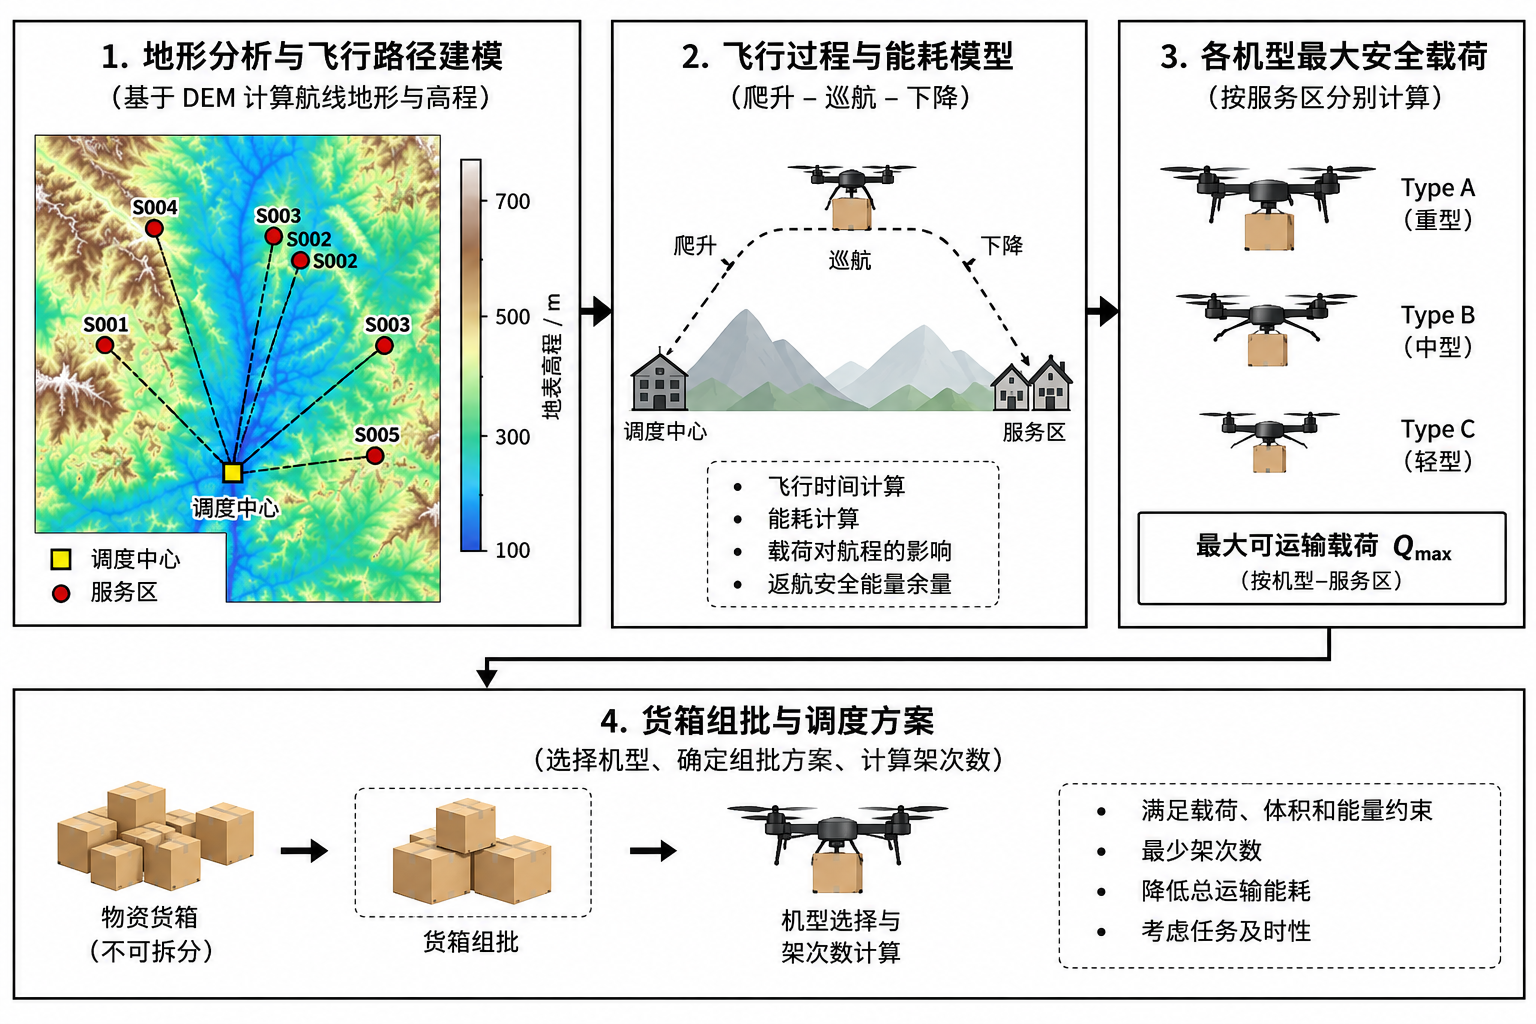
\includegraphics[width=0.8\textwidth]{figures/Q1_FIg1.png}
  \caption{问题一建模与求解总框架}
  \label{fig:problem1_flow}
\end{figure}

图~\ref{fig:problem1_flow}将问题一划分为“地形与航段预处理、单架次物理模型、安全载荷计算、离散组批优化”四个环节。前两步给出任意机型在任意服务区的时间和能耗计算口径，后两步在此基础上完成运输能力评估与货箱分批，最终输出可直接用于后续调度问题的单架次可行方案。

\subsection{基本约定}
（1）每一运输架次均采用 $O_{01}\to S_i\to O_{01}$ 的直接往返形式，只服务一个服务区；同一服务区允许使用多个架次完成配送，但不得跨服务区组批。

（2）任意两个任务节点之间的水平航迹取两节点连线；巡航海拔由该连线经过的30\,m DEM像元最高地形高程加50\,m安全净空确定。

（3）$O_{01}$ 的作业高度取地面海拔，服务区作业高度取地面海拔以上30\,m；每个航段均按“爬升--水平巡航--下降”三个阶段计算飞行时间。

（4）按题设统一能耗口径，下降阶段不单独计入附加势能消耗；运输总能耗由载荷相关的水平航程能耗与爬升附加能耗构成。

（5）问题一不考虑实体无人机数量、共享电池数量及充电周转，只考察单架次物理可行性与货箱组批；货箱不可拆分且每个货箱只能被安排一次。

\FloatBarrier

\subsection{航段时间与能耗模型}

\subsubsection{基于DEM的航段净空模型}
对于节点 $i$ 到节点 $j$ 的运输航段，沿节点连线检查其穿越的DEM像元。设这些像元的最高地形高程为 $\max(h_k)$，则计划巡航海拔为

\begin{equation}
H_{ij}=\max_{k\in L_{ij}}h_k+50,
\label{eq:q1-clearance}
\end{equation}
其中，$L_{ij}$ 表示航段 $i\to j$ 穿越的DEM像元集合。设节点 $i$、$j$ 的实际作业海拔分别为 $z_i^o$、$z_j^o$，则爬升高度和下降高度分别为

\begin{equation}
h_{ij}^{\uparrow}=H_{ij}-z_i^o,\qquad
h_{ij}^{\downarrow}=H_{ij}-z_j^o.
\label{eq:q1-vertical-height}
\end{equation}

该处理把沿线最高地形直接转化为爬升需求，使距离相近但地形条件不同的服务区能够得到不同的时间与能耗结果，避免仅按平面距离估计运输能力。

\subsubsection{载荷相关等效航程与运输能耗}
题目给出了各机型的空载标准航程与满载标准航程。按题设统一计算规则，机型 $g$ 在载荷 $q$ 下的等效航程为

\begin{equation}
R_g(q)=R_g^0-\bigl(R_g^0-R_g^F\bigr)
\left(\frac{q}{Q_g}\right)^{3/2},\qquad 0\le q\le Q_g.
\label{eq:q1-range}
\end{equation}

机型 $g$ 携带载荷 $q$ 执行航段 $i\to j$ 时，水平巡航能耗按“单组电池能量$\times$航段距离/等效航程”折算，并叠加爬升势能项，得到

\begin{equation}
E_{ij}(g\mid q)
=E_g\frac{d_{ij}}{R_g(q)}
+\frac{(m_g+q)g_0h_{ij}^{\uparrow}}{\eta_g\,3.6\times10^6}.
\label{eq:q1-segment-energy}
\end{equation}

式中 $g_0=9.81\,\mathrm{m}/\mathrm{s}^2$；第二项除以 $3.6\times10^6$ 将焦耳换算为kWh。由于题目规定下降阶段不单独计算附加势能消耗，故式~\eqref{eq:q1-segment-energy}仅包含水平巡航和爬升两部分。

\subsubsection{飞行时间与单架次作业时间}
机型 $g$ 在航段 $i\to j$ 上的飞行时间由爬升、巡航和下降三个阶段组成：

\begin{equation}
t_{ij}(g)
=\frac{h_{ij}^{\uparrow}}{v_g^{\uparrow}}
+\frac{d_{ij}}{v_g}
+\frac{h_{ij}^{\downarrow}}{v_g^{\downarrow}}.
\label{eq:q1-flight-time}
\end{equation}

若问题一的某一直接往返架次包含 $n$ 个货箱，则累计作业时间还包括起飞准备、逐箱装载、服务区交接和逐箱卸载：

\begin{equation}
\begin{aligned}
T_p={}&t_g^{\mathrm{prep}}+n\,t_g^{\mathrm{load}}
+t_{O_{01},i}(g)+t_{i,O_{01}}(g)\\
&+t_g^{\mathrm{service}}+n\,t_g^{\mathrm{unload}}.
\end{aligned}
\label{eq:q1-operation-time}
\end{equation}

需要说明的是，$T_p$ 为单架次从准备到返航的作业时长；后文的“累计作业时间”是各架次 $T_p$ 的求和，不等同于多架无人机并行执行时的任务完工时间。

\subsection{单点往返最大安全载荷模型}
问题一首先要求计算三种机型在不同服务区执行直接往返任务时的最大安全载荷。起飞时无人机携带全部货物，到达服务区后完成投送，返航阶段按空载计算。因此，机型 $g$ 向服务区 $S_i$ 运送载荷 $q$ 时的一次往返总能耗为

\begin{equation}
E_{gi}^{\mathrm{rt}}(q)
=E_{O_{01},i}(g\mid q)+E_{i,O_{01}}(g\mid0).
\label{eq:q1-roundtrip-energy}
\end{equation}

为保证返航安全，任务结束时必须至少保留 $p_g$ 比例的电量，即

\begin{equation}
E_{gi}^{\mathrm{rt}}(q)\le(1-p_g)E_g.
\label{eq:q1-energy-limit}
\end{equation}

因此，机型 $g$ 在服务区 $S_i$ 的最大安全载荷定义为

\begin{equation}
q_{gi}^{\mathrm{safe}}=
\max\left\{q\;\middle|\;
0\le q\le Q_g,\quad
E_{gi}^{\mathrm{rt}}(q)\le(1-p_g)E_g
\right\}.
\label{eq:q1-safe-payload}
\end{equation}

由式~\eqref{eq:q1-range}和式~\eqref{eq:q1-segment-energy}可知，在给定航段上 $E_{gi}^{\mathrm{rt}}(q)$ 随载荷增加单调不减。若额定载荷 $Q_g$ 已满足式~\eqref{eq:q1-energy-limit}，则 $q_{gi}^{\mathrm{safe}}=Q_g$；否则主程序在 $[0,Q_g]$ 上采用Brent法求解唯一临界载荷。若 $q=0$ 时仍不能满足返航余量，则判定该“机型--服务区”组合在当前余量下不可达。

为直观说明式~\eqref{eq:q1-safe-payload}所刻画的能力边界，以S008的去、返程爬升参数为固定条件，在20\%返航安全余量下计算不同载荷对应的最大可行单程水平距离，结果见图~\ref{fig:q1-payload-distance}。

\begin{figure}[htbp!]
  \centering
  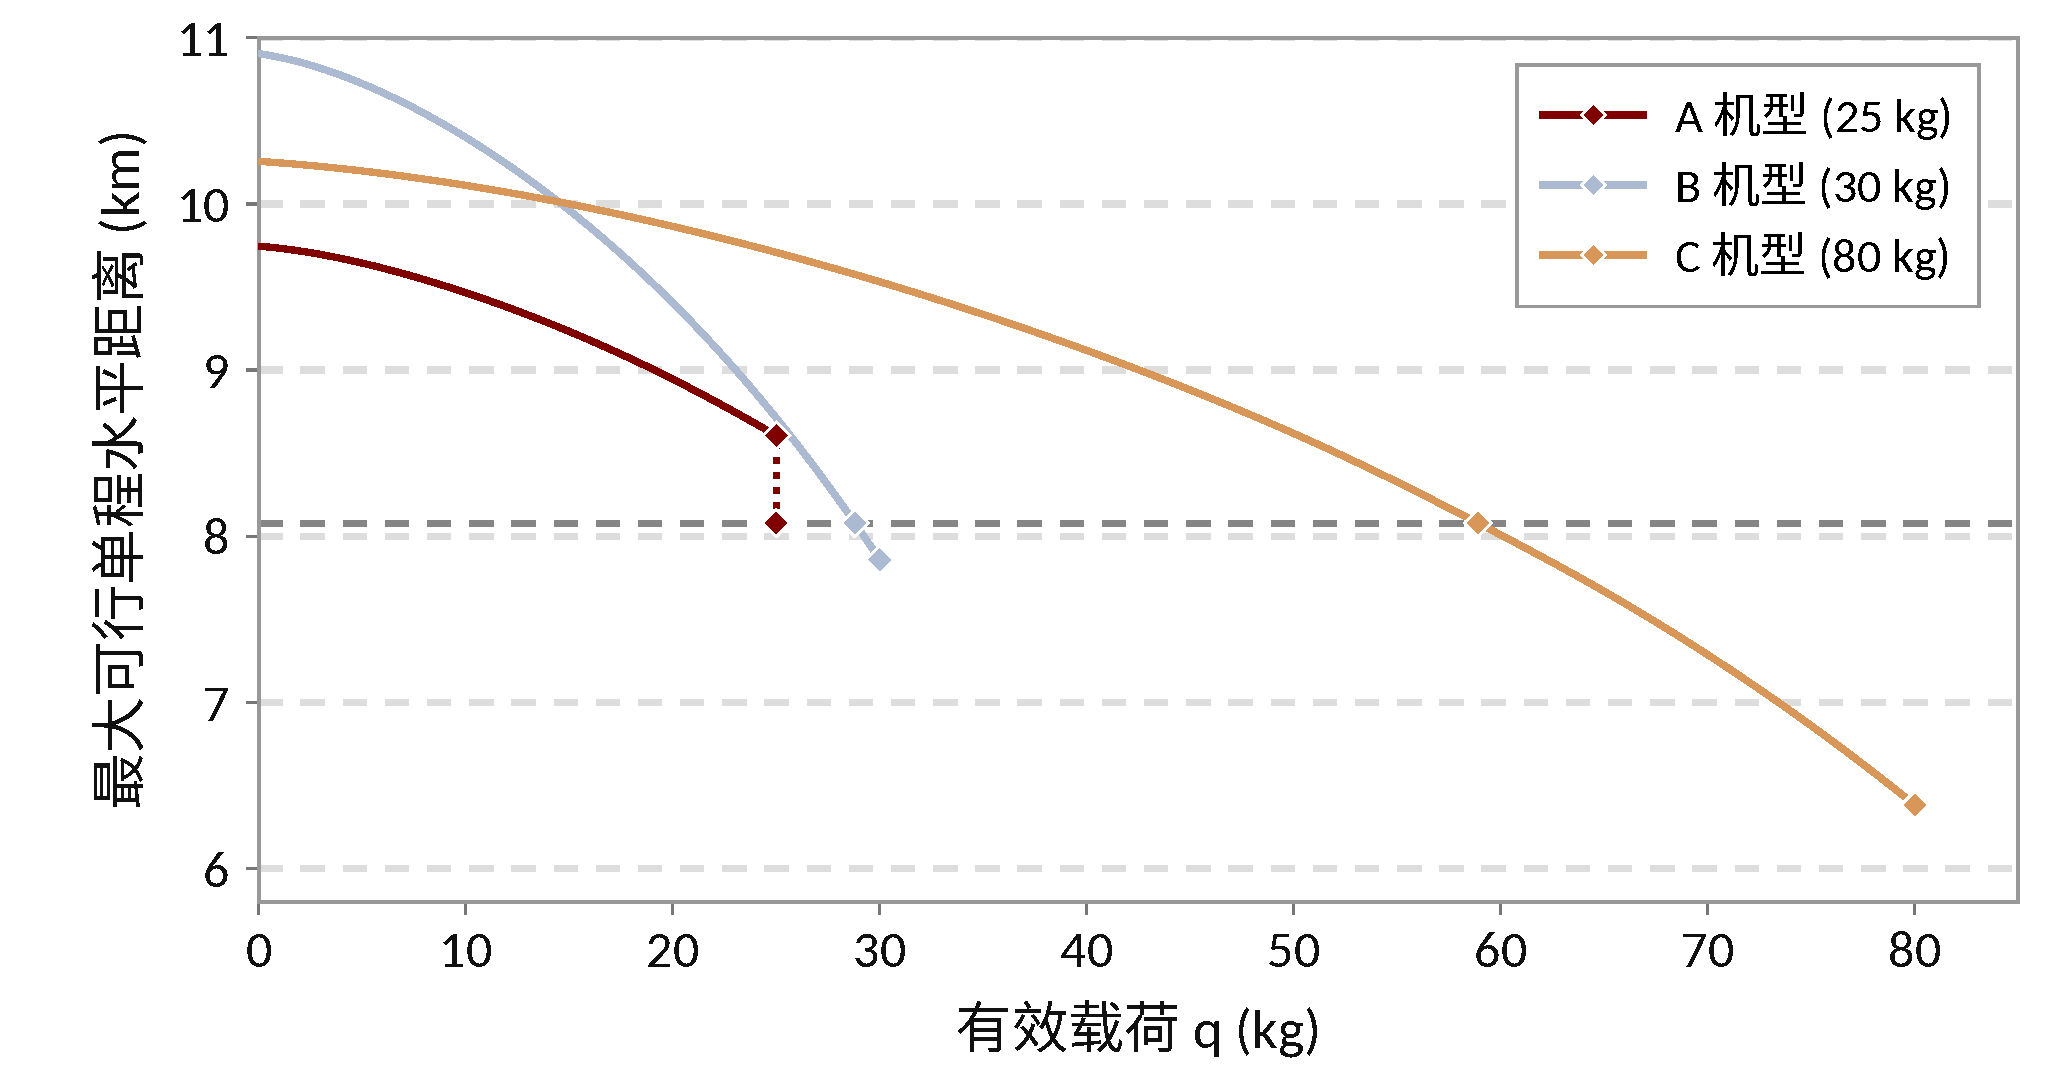
\includegraphics[width=0.8\textwidth]{figures/payload_distance.pdf}
  \caption{固定S008爬升条件下三种机型的载荷--距离能量可行边界（20\%返航安全余量）}
  \label{fig:q1-payload-distance}
\end{figure}

图~\ref{fig:q1-payload-distance}显示，随着有效载荷增加，可由同一能量预算支持的水平距离持续缩短。若某机型的能量边界在额定载荷范围内与S008实际单程距离相交，则交点横坐标给出能量约束下的临界载荷；若整个额定载荷区间均满足往返能量约束，则最大安全载荷由额定载质量截断。该图仅用于解释模型关系：横向改变距离时保持S008的爬升参数不变，因此不应把曲线解释为重新采样DEM后的真实地理服务半径，也不属于Pareto前沿。

\subsection{货箱组批优化模型}

\subsubsection{可行组批约束}
对服务区 $S_i$ 的货箱集合 $B_i$，任意候选批次 $p\subseteq B_i$ 选择一种机型 $g_p$。设该批次的货箱总质量和总体积分别为 $M_p$ 与 $V_p$，则必须满足

\begin{equation}
M_p=\sum_{b\in p}m_b\le Q_{g_p},\qquad
V_p=\sum_{b\in p}v_b\le V_{g_p}.
\label{eq:q1-capacity}
\end{equation}

同时，候选批次还必须满足返航安全能量约束

\begin{equation}
E_{O_{01},i}(g_p\mid M_p)
+E_{i,O_{01}}(g_p\mid0)
\le(1-p_{g_p})E_{g_p}.
\label{eq:q1-batch-energy}
\end{equation}

式~\eqref{eq:q1-capacity}和式~\eqref{eq:q1-batch-energy}共同决定一个货箱组合是否可由某一机型完成。最大安全载荷只是对连续质量变量给出的上限，实际货箱不可拆分，且还受到装载体积约束，因此不能仅依据 $q_{gi}^{\mathrm{safe}}$ 进行贪心装箱。

\subsubsection{多目标优化与优先关系}
题目要求在完成全部货箱交付的前提下综合考虑往返架次数、总运输能耗和累计作业时间。考虑到问题一不涉及多机并行排程，减少架次数可以直接减少运输批次和重复准备、交接环节，本文采用字典序目标：先最小化架次数，再在最少架次方案中最小化总运输能耗，最后最小化累计作业时间，即

\begin{equation}
\min_{\mathrm{lex}}\;(N,E,T).
\label{eq:q1-objective}
\end{equation}

其中
\[
N=\sum_p x_p,\qquad
E=\sum_p E_p x_p,\qquad
T=\sum_p T_p x_p,
\]
$x_p\in\{0,1\}$ 表示可行组批模式 $p$ 是否被选用。每个货箱必须且只能出现一次：

\begin{equation}
\sum_{p:\,b\in p}x_p=1,\qquad \forall b\in B_i.
\label{eq:q1-exact-cover}
\end{equation}

后文同时以“能耗优先”和“累计作业时间优先”重新求解，比较不同优先关系对最终方案的影响，以避免仅凭主观判断确定目标次序。

\subsection{精确动态规划求解方法}
由于问题一禁止跨服务区组批，且不考虑跨架次资源竞争，15个服务区可以独立精确求解。为降低状态维度，将同一服务区内“物资类别、单箱质量、单箱体积”完全相同的货箱归为一类。问题一不包含逐箱时限约束，因此该聚合不会损失可行性。

设服务区 $S_i$ 共有 $K$ 类货箱，第 $k$ 类数量为 $n_k$，定义状态向量
$\boldsymbol{x}=(x_1,x_2,\ldots,x_K)$，其中 $x_k$ 表示尚未分配的第 $k$ 类货箱数量。首先枚举所有满足质量、体积和返航安全能量约束的可行模式 $p$，记录其数量向量 $\boldsymbol{c}_p$、机型 $g_p$、能耗 $E_p$ 和作业时间 $T_p$。令 $F(\boldsymbol{x})$ 表示完成状态 $\boldsymbol{x}$ 中全部剩余货箱所需的最优代价向量，则

\begin{equation}
F(\boldsymbol{x})=
\min_{\mathrm{lex}}\left\{
(1,E_p,T_p)+F(\boldsymbol{x}-\boldsymbol{c}_p)
\;\middle|\;
\boldsymbol{0}<\boldsymbol{c}_p\le\boldsymbol{x},\ p\text{ 可行}
\right\},
\label{eq:q1-dp}
\end{equation}

\begin{equation}
F(\boldsymbol{0})=(0,0,0).
\label{eq:q1-dp-initial}
\end{equation}

采用记忆化搜索保存已计算状态，避免重复计算。由于各服务区的决策变量、覆盖约束和代价均相互独立，而三个目标又对服务区结果可加，因此逐区按同一字典序取得最优解并求和，即得到问题一的全局字典序最优解。

为降低对单一算法实现的依赖，本文另外以同一批可行组批模式建立0--1整数规划：先独立求各服务区的最少架次数，再固定该架次数求最小运输能耗。该模型只用于交叉验证，不参与主方案生成。

\subsection{计算结果与分析}
本节结果均由题目给定的节点坐标、30\,m DEM、货箱数据和运输无人机参数按上述模型计算得到，属于题设数据上的数值实验结果。默认方案使用20\%返航安全余量；敏感性实验仅改变返航安全余量，其余输入参数和求解口径保持不变。

\subsubsection{三种机型的最大安全载荷}
为说明地形条件和载荷变化如何共同影响无人机的安全运输能力，图~\ref{fig:fig1}选取 S001、S004 和 S008 三个具有代表性的服务区进行比较。S001 对三种机型均未形成明显的能量约束，S004 主要限制 C 型无人机，而 S008 同时对 B、C 两型形成约束。图中上排给出三个服务区对应航线的地形与巡航高度关系，下排给出相同地形条件下三种机型的往返运输能耗随有效载荷变化的结果。虚线表示在 20\% 返航安全余量下各机型允许使用的最大能量，曲线与能量边界的关系决定相应机型的最大安全载荷。
\begin{figure}[htbp!]
  \centering
  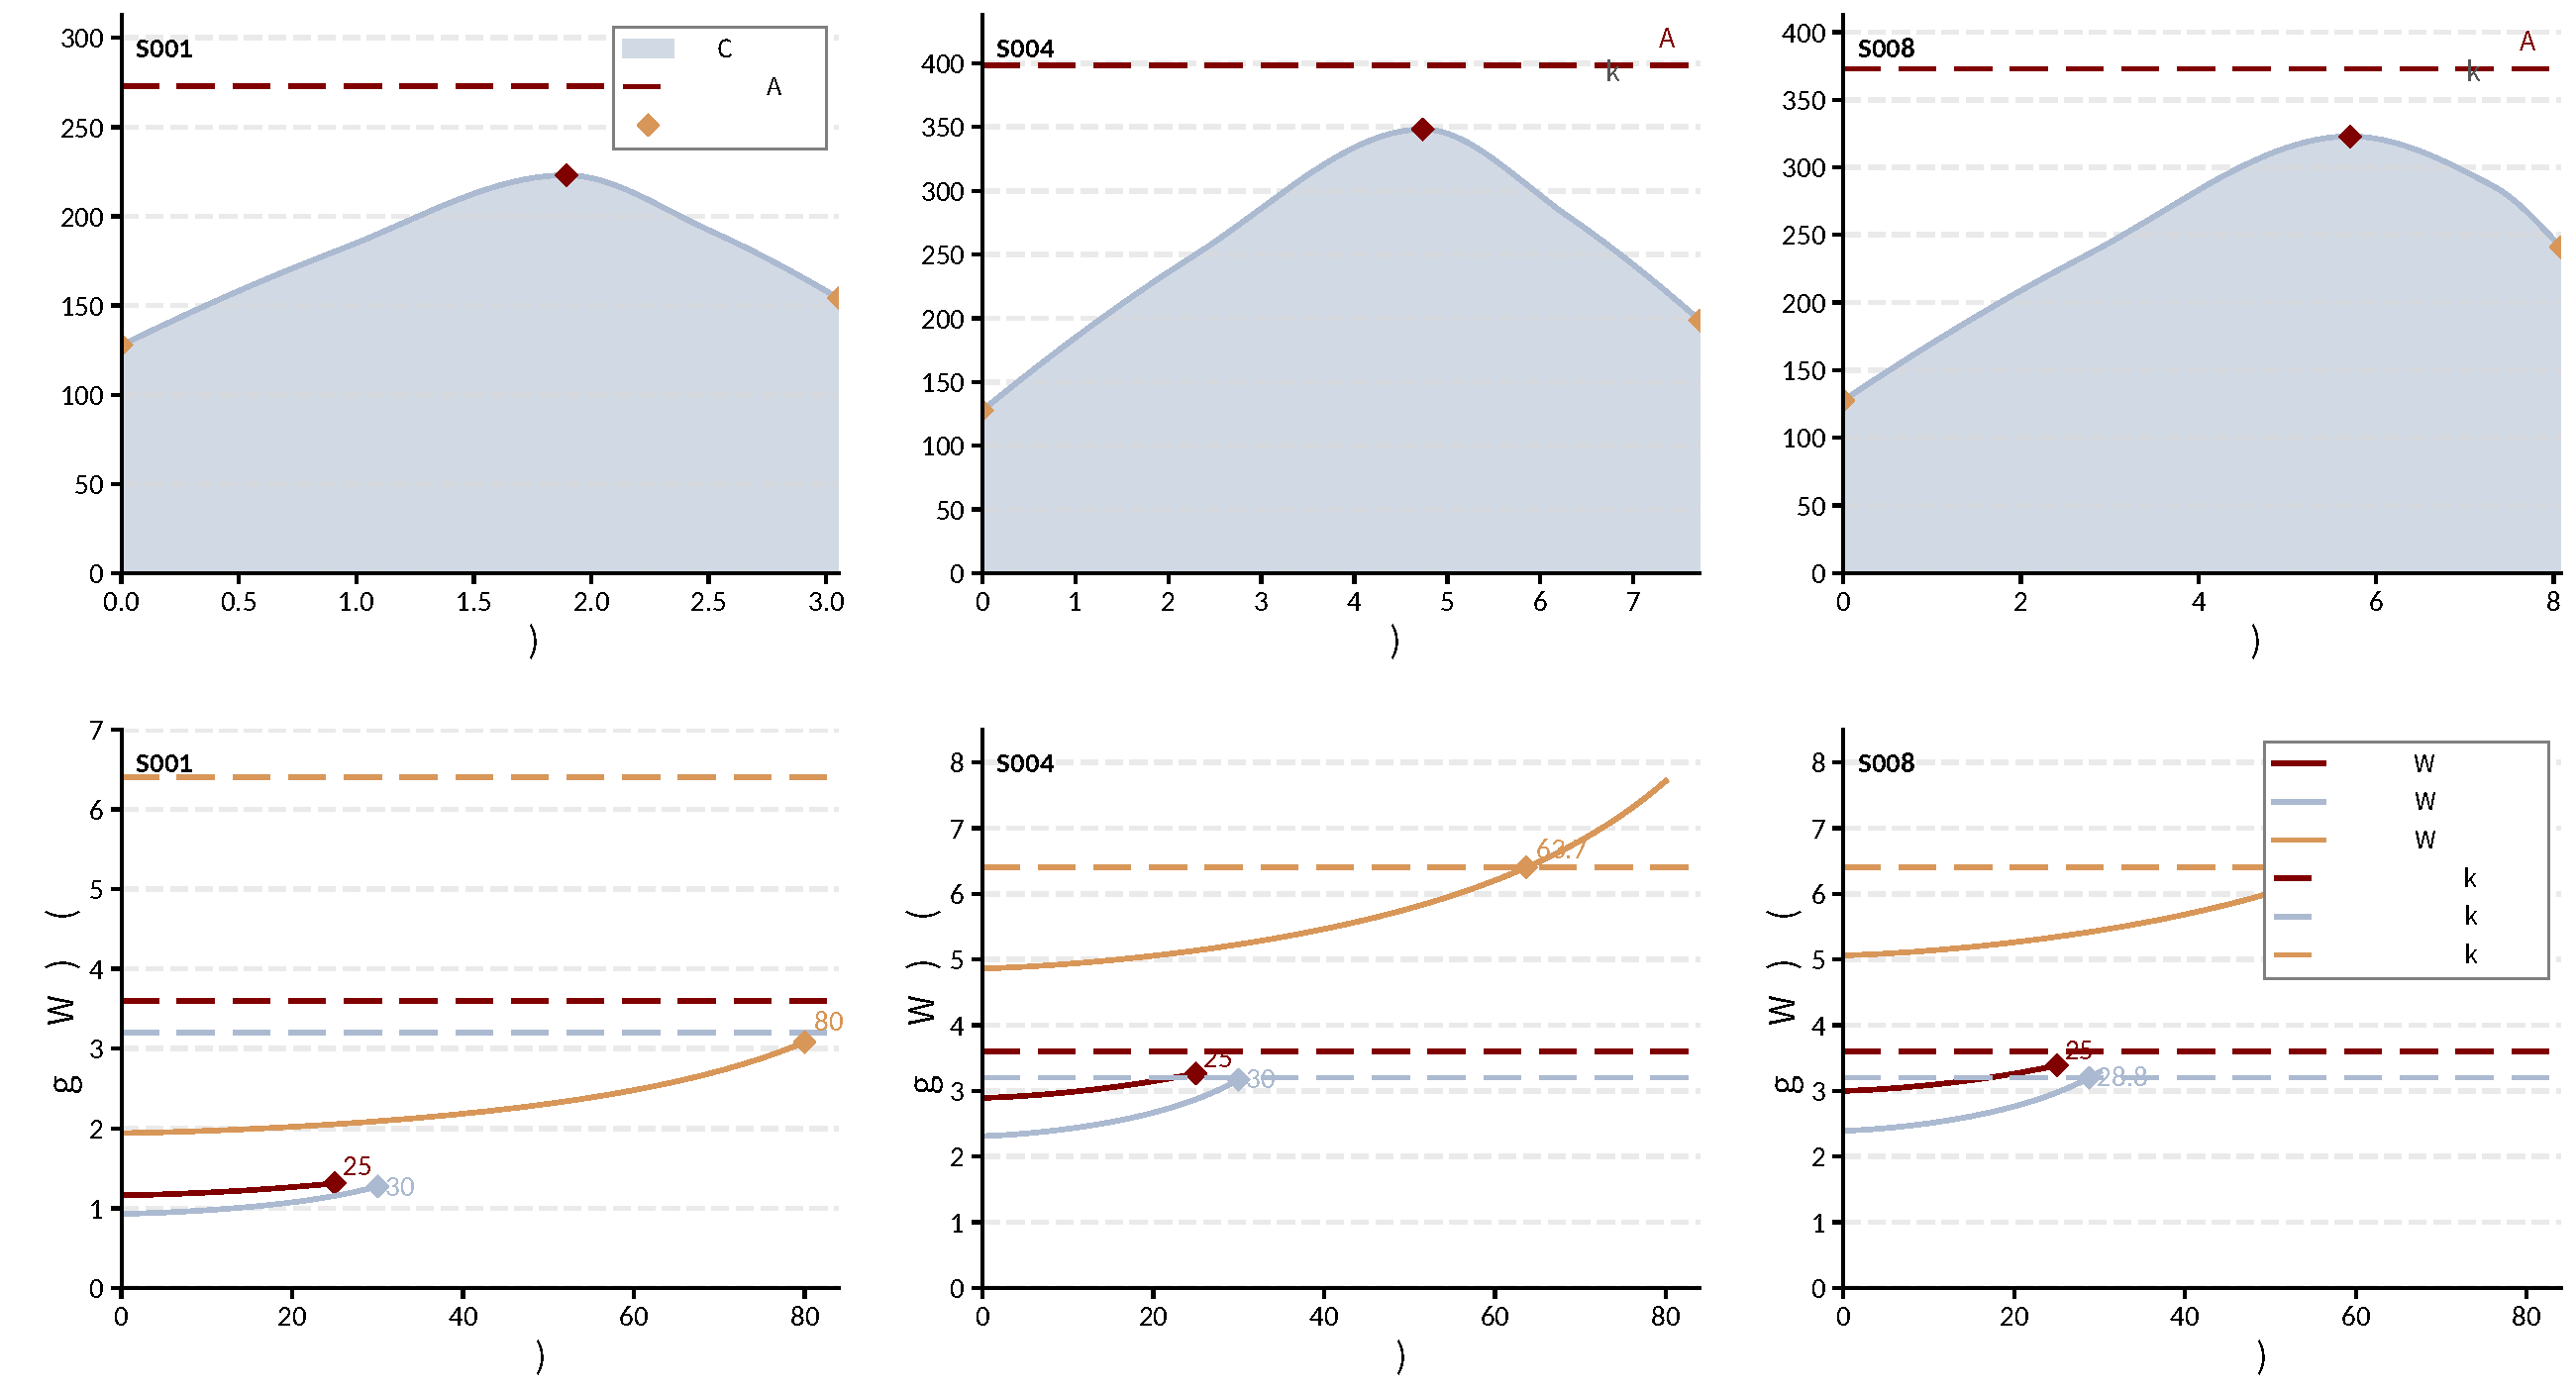
\includegraphics[width=0.8\textwidth]{figures/问题一_典型服务区地形与载荷能耗关系.pdf}
  \caption{典型服务区的地形约束与载荷—能耗关系}
  \label{fig:fig1}
\end{figure}
可以看出，不同服务区的运输能力差异并非由水平距离单独决定，而是由航程、地形爬升需求和载荷引起的等效航程衰减共同造成。以 S001 为例，三种机型在额定载荷下均未触及安全能量上限，因此最大安全载荷分别保持为 25、30 和 80 kg；在 S004，C 型能耗曲线在达到额定载荷前已与安全能量边界相交，其最大安全载荷下降至 63.697 kg；S008 的约束进一步增强，B、C 两型的最大安全载荷分别降至 28.801 kg 和 58.904 kg。在题目默认的20\%返航安全余量下，三种机型对15个服务区的最大安全载荷如图~\ref{fig:q1-safe-payload}和表~\ref{tab:q1-safe-payload}所示。

\begin{figure}[htbp!]
  \centering
  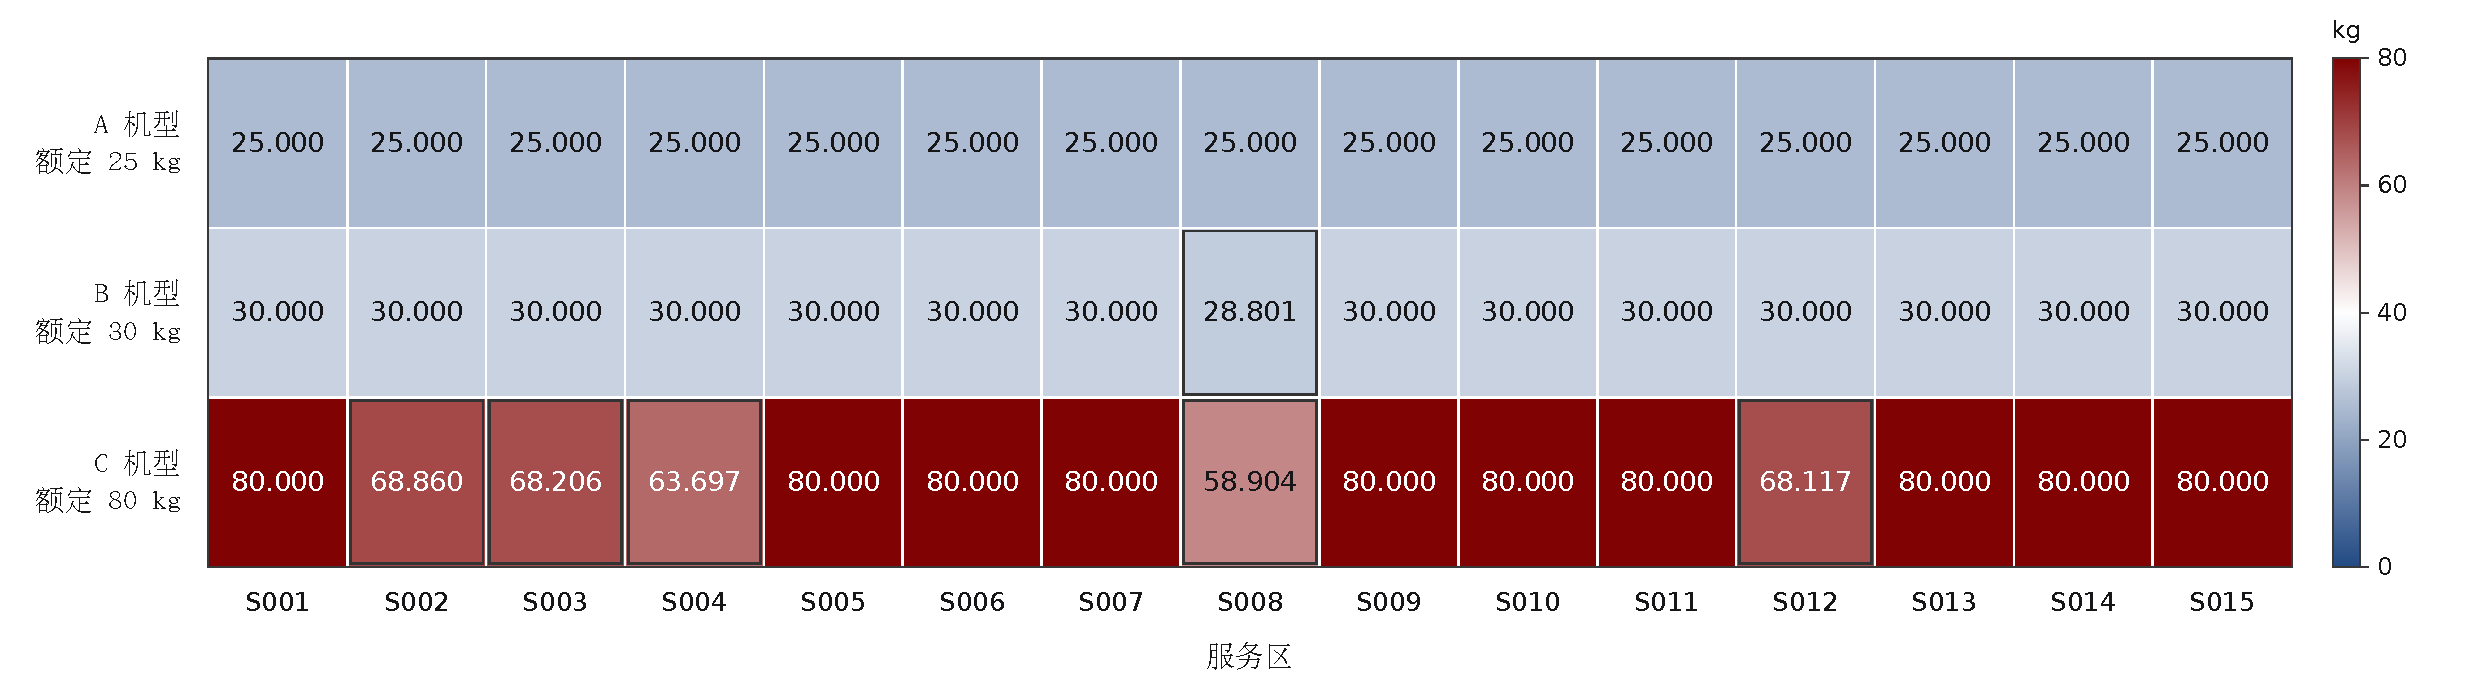
\includegraphics[width=0.8\textwidth]{figures/3.2.pdf}
  \caption{20\%返航安全余量下三种机型的最大安全载荷热力图}
  \label{fig:q1-safe-payload}
\end{figure}

图~\ref{fig:q1-safe-payload}以颜色表示安全载荷大小，格内数值为对应“机型--服务区”的计算结果。A型在全部服务区均达到25\,kg额定载荷；B型仅S008受能量约束，最大安全载荷为28.801\,kg；C型在S002、S003、S004、S008和S012低于80\,kg额定上限，说明重载机型在较不利航段上更容易由能量约束而非额定载质量决定运输能力。

\begin{table}[htbp!]
  \centering
  \small
  \setlength{\tabcolsep}{5pt}
  \renewcommand{\arraystretch}{1.15}
  \caption{20\%返航安全余量下各服务区最大安全载荷（kg）}
  \label{tab:q1-safe-payload}
  \begin{tabular*}{0.75\linewidth}{@{\extracolsep{\fill}}crrr@{}}
    \toprule
    服务区 & A型 & B型 & C型 \\
    \midrule
    S001 & 25.000 & 30.000 & 80.000 \\
    S002 & 25.000 & 30.000 & 68.860 \\
    S003 & 25.000 & 30.000 & 68.206 \\
    S004 & 25.000 & 30.000 & 63.697 \\
    S005 & 25.000 & 30.000 & 80.000 \\
    S006 & 25.000 & 30.000 & 80.000 \\
    S007 & 25.000 & 30.000 & 80.000 \\
    S008 & 25.000 & 28.801 & 58.904 \\
    S009 & 25.000 & 30.000 & 80.000 \\
    S010 & 25.000 & 30.000 & 80.000 \\
    S011 & 25.000 & 30.000 & 80.000 \\
    S012 & 25.000 & 30.000 & 68.117 \\
    S013 & 25.000 & 30.000 & 80.000 \\
    S014 & 25.000 & 30.000 & 80.000 \\
    S015 & 25.000 & 30.000 & 80.000 \\
    \bottomrule
  \end{tabular*}
\end{table}

表~\ref{tab:q1-safe-payload}给出用于后续组批的精确数值。对C型而言，S008的安全载荷最低，仅58.904\,kg；S002、S003、S004和S012也低于额定上限。S008同时对B、C两型形成约束，因此选作后续返航余量敏感性分析的代表性困难服务区。

\subsubsection{最优货箱组批方案}
在20\%返航安全余量和“架次数--能耗--累计作业时间”字典序目标下，80个货箱共被划分为18个直接往返架次，总运输能耗为59.1313\,kWh，累计作业时间为9.104\,h，其中纯飞行时间为5.358\,h。最终使用B型9架次、C型9架次，A型未被采用。各架次货箱组成如图~\ref{fig:q1-batching}所示，完整数值见表~\ref{tab:q1-batching}。

\begin{figure}[htbp!]
  \centering
  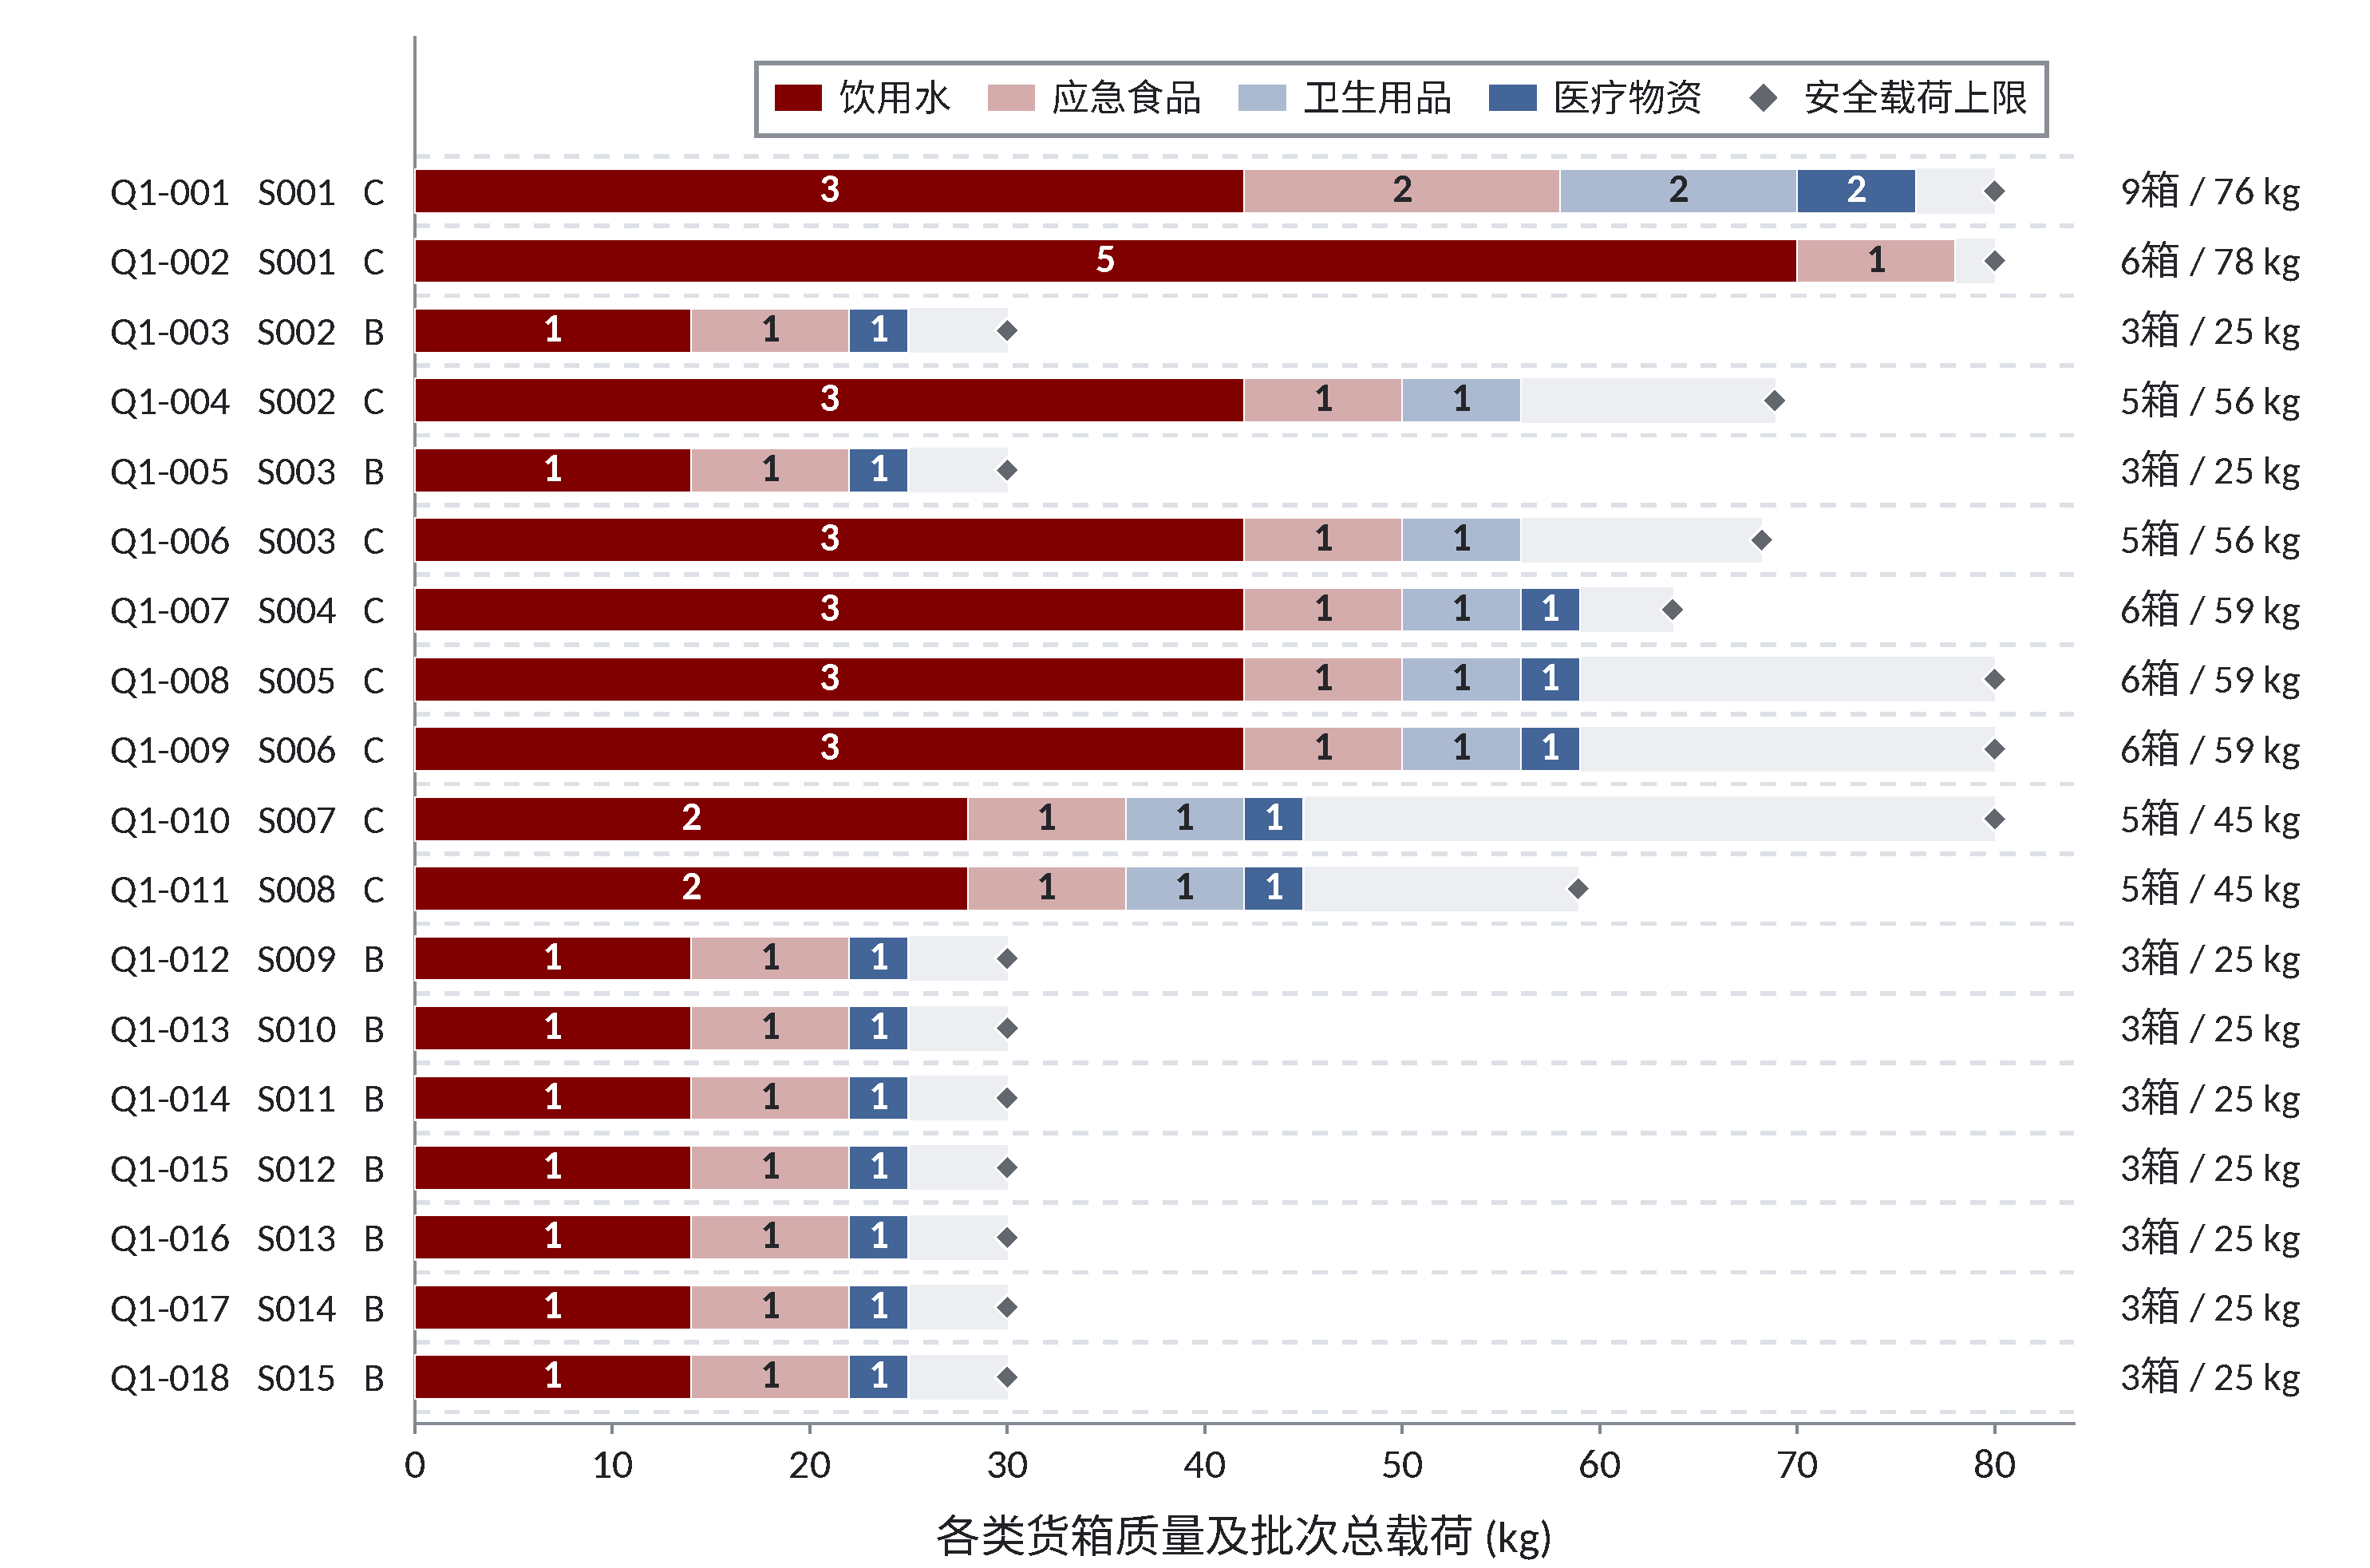
\includegraphics[width=0.8\textwidth]{figures/flight_loading_red_blue.pdf}
  \caption{问题一18架次货箱组成及机型分配}
  \label{fig:q1-batching}
\end{figure}

图~\ref{fig:q1-batching}中每一条横条对应一个实际运输架次，不同色块表示各类货箱的质量贡献，条末给出该架次箱数与总载荷；安全载荷上限用于判断该批次在对应服务区是否满足连续质量意义下的运输能力约束。该图用于展示组批结构，能耗、体积和返航SOC等精确数值以表~\ref{tab:q1-batching}为准。

\FloatBarrier
\begingroup
\small
\setlength{\tabcolsep}{4pt}
\renewcommand{\arraystretch}{1.2}
\setlength{\LTleft}{\fill}
\setlength{\LTright}{\fill}
\begin{longtable}{@{}lcclrrrrr@{}}
  \caption{问题一最优组批与运输结果}\label{tab:q1-batching}\\
  \toprule
    架次 & 服务区 & 机型 & 货箱组成 & \shortstack{载荷\\ /$\mathrm{kg}$} & \shortstack{体积\\ /$\mathrm{m}^{3}$} & \shortstack{能耗\\ /$\mathrm{kWh}$} & \shortstack{作业时间\\ /$\mathrm{min}$} & \shortstack{返航SOC\\ /$\%$} \\
  \midrule
  \endfirsthead
  \multicolumn{9}{c}{表~\thetable（续）}\\
  \toprule
    架次 & 服务区 & 机型 & 货箱组成 & \shortstack{载荷\\ /$\mathrm{kg}$} & \shortstack{体积\\ /$\mathrm{m}^{3}$} & \shortstack{能耗\\ /$\mathrm{kWh}$} & \shortstack{作业时间\\ /$\mathrm{min}$} & \shortstack{返航SOC\\ /$\%$} \\
  \midrule
  \endhead
  \midrule
  \multicolumn{9}{r}{\footnotesize 续下页}\\
  \endfoot
  \bottomrule
  \endlastfoot
    Q1-001 & S001 & C & \shortstack[l]{\strut $\mathrm{FOD}\times2$\quad $\mathrm{HYG}\times2$\\\strut $\mathrm{MED}\times2$\quad $\mathrm{WAT}\times3$} & 76 & 0.231 & 2.918 & 28.20 & 63.5 \\[3pt]
    Q1-002 & S001 & C & \shortstack[l]{\strut $\mathrm{FOD}\times1$\quad $\mathrm{WAT}\times5$} & 78 & 0.163 & 2.996 & 24.90 & 62.6 \\[3pt]
    Q1-003 & S002 & B & \shortstack[l]{\strut $\mathrm{FOD}\times1$\quad $\mathrm{MED}\times1$\\\strut $\mathrm{WAT}\times1$} & 25 & 0.067 & 2.713 & 30.28 & 32.2 \\[3pt]
    Q1-004 & S002 & C & \shortstack[l]{\strut $\mathrm{FOD}\times1$\quad $\mathrm{HYG}\times1$\\\strut $\mathrm{WAT}\times3$} & 56 & 0.144 & 5.721 & 34.03 & 28.5 \\[3pt]
    Q1-005 & S003 & B & \shortstack[l]{\strut $\mathrm{FOD}\times1$\quad $\mathrm{MED}\times1$\\\strut $\mathrm{WAT}\times1$} & 25 & 0.067 & 2.780 & 34.68 & 30.5 \\[3pt]
    Q1-006 & S003 & C & \shortstack[l]{\strut $\mathrm{FOD}\times1$\quad $\mathrm{HYG}\times1$\\\strut $\mathrm{WAT}\times3$} & 56 & 0.144 & 5.765 & 39.50 & 27.9 \\[3pt]
    Q1-007 & S004 & C & \shortstack[l]{\strut $\mathrm{FOD}\times1$\quad $\mathrm{HYG}\times1$\\\strut $\mathrm{MED}\times1$\quad $\mathrm{WAT}\times3$} & 59 & 0.156 & 6.153 & 38.35 & 23.1 \\[3pt]
    Q1-008 & S005 & C & \shortstack[l]{\strut $\mathrm{FOD}\times1$\quad $\mathrm{HYG}\times1$\\\strut $\mathrm{MED}\times1$\quad $\mathrm{WAT}\times3$} & 59 & 0.156 & 4.222 & 31.29 & 47.2 \\[3pt]
    Q1-009 & S006 & C & \shortstack[l]{\strut $\mathrm{FOD}\times1$\quad $\mathrm{HYG}\times1$\\\strut $\mathrm{MED}\times1$\quad $\mathrm{WAT}\times3$} & 59 & 0.156 & 2.598 & 26.03 & 67.5 \\[3pt]
    Q1-010 & S007 & C & \shortstack[l]{\strut $\mathrm{FOD}\times1$\quad $\mathrm{HYG}\times1$\\\strut $\mathrm{MED}\times1$\quad $\mathrm{WAT}\times2$} & 45 & 0.129 & 3.411 & 31.79 & 57.4 \\[3pt]
    Q1-011 & S008 & C & \shortstack[l]{\strut $\mathrm{FOD}\times1$\quad $\mathrm{HYG}\times1$\\\strut $\mathrm{MED}\times1$\quad $\mathrm{WAT}\times2$} & 45 & 0.129 & 5.836 & 36.66 & 27.0 \\[3pt]
    Q1-012 & S009 & B & \shortstack[l]{\strut $\mathrm{FOD}\times1$\quad $\mathrm{MED}\times1$\\\strut $\mathrm{WAT}\times1$} & 25 & 0.067 & 2.096 & 25.97 & 47.6 \\[3pt]
    Q1-013 & S010 & B & \shortstack[l]{\strut $\mathrm{FOD}\times1$\quad $\mathrm{MED}\times1$\\\strut $\mathrm{WAT}\times1$} & 25 & 0.067 & 1.823 & 25.92 & 54.4 \\[3pt]
    Q1-014 & S011 & B & \shortstack[l]{\strut $\mathrm{FOD}\times1$\quad $\mathrm{MED}\times1$\\\strut $\mathrm{WAT}\times1$} & 25 & 0.067 & 1.074 & 19.81 & 73.2 \\[3pt]
    Q1-015 & S012 & B & \shortstack[l]{\strut $\mathrm{FOD}\times1$\quad $\mathrm{MED}\times1$\\\strut $\mathrm{WAT}\times1$} & 25 & 0.067 & 2.752 & 32.05 & 31.2 \\[3pt]
    Q1-016 & S013 & B & \shortstack[l]{\strut $\mathrm{FOD}\times1$\quad $\mathrm{MED}\times1$\\\strut $\mathrm{WAT}\times1$} & 25 & 0.067 & 1.825 & 25.17 & 54.4 \\[3pt]
    Q1-017 & S014 & B & \shortstack[l]{\strut $\mathrm{FOD}\times1$\quad $\mathrm{MED}\times1$\\\strut $\mathrm{WAT}\times1$} & 25 & 0.067 & 2.140 & 31.16 & 46.5 \\[3pt]
    Q1-018 & S015 & B & \shortstack[l]{\strut $\mathrm{FOD}\times1$\quad $\mathrm{MED}\times1$\\\strut $\mathrm{WAT}\times1$} & 25 & 0.067 & 2.307 & 30.47 & 42.3 \\[3pt]
\end{longtable}
\endgroup

\noindent\textit{注：}同一服务区内同类别货箱的质量与体积参数一致，因此“货箱组成”按类别计数表示；FOD、HYG、MED、WAT分别表示应急食品、生活卫生用品、医疗物资和饮用水。

表~\ref{tab:q1-batching}显示，只有S001、S002和S003需要2个架次，其余12个服务区均可在1个架次内完成。S001总需求质量为154\,kg，要在最少的2个架次内完成只能使用C型，两架次载荷分别为76\,kg和78\,kg；S002、S003均采用“25\,kg的B型架次+56\,kg的C型架次”。S004--S008由C型单架次完成，S009--S015由B型单架次完成。

A型未进入最终最优方案并不意味着其单点往返不可行。实际组批还受货箱不可拆分和体积约束影响。例如“饮用水14\,kg+医疗物资3\,kg+应急食品8\,kg”的组合总质量恰为25\,kg，但总体积为0.067\,m$^3$，超过A型0.060\,m$^3$的装载体积，而B型0.073\,m$^3$可以容纳。该例说明，仅依据额定载质量进行组批会高估A型在离散货箱组合中的适用范围。

\subsubsection{架次数、能耗与作业时间的权衡}
为检验字典序优先关系是否合理，分别以能耗和累计作业时间作为第一目标重新求解，并与本文方案比较，结果见表~\ref{tab:q1-objective-comparison}和图~\ref{fig:q1-objective-comparison}。

\begin{table}[htbp!]
  \centering
  \small
  \setlength{\tabcolsep}{5pt}
  \renewcommand{\arraystretch}{1.15}
  \caption{不同优化优先级下的结果对比}
  \label{tab:q1-objective-comparison}
  \begin{tabular*}{\linewidth}{@{\extracolsep{\fill}}lrrrrrr@{}}
    \toprule
    优化策略 & 架次数 & \shortstack{总能耗\\ /$\mathrm{kWh}$} & \shortstack{累计作业时间\\ /$\mathrm{h}$} & A型 & B型 & C型 \\
    \midrule
    架次数优先（本文） & 18 & 59.1313 & 9.104 & 0 & 9 & 9 \\
    能耗优先 & 19 & 59.0339 & 9.567 & 0 & 11 & 8 \\
    时间优先 & 18 & 59.1313 & 9.104 & 0 & 9 & 9 \\
    \bottomrule
  \end{tabular*}
\end{table}

\begin{figure}[htbp!]
  \centering
  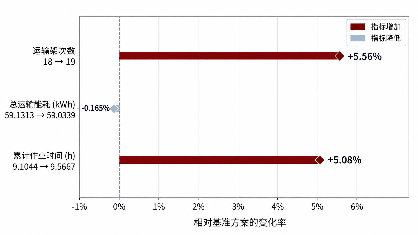
\includegraphics[width=0.8\textwidth]{figures/运输与能耗变化率对比图.pdf}
  \caption{能耗优先方案相对本文方案的指标变化}
  \label{fig:q1-objective-comparison}
\end{figure}

表~\ref{tab:q1-objective-comparison}给出三个目标优先关系下的绝对结果，图~\ref{fig:q1-objective-comparison}进一步以本文方案为基准展示采用“能耗优先”后的相对变化。能耗优先时，总能耗由59.1313\,kWh降至59.0339\,kWh，仅减少0.165\%；与此同时，架次数由18增至19，增加5.56\%，累计作业时间由9.104\,h增至9.567\,h，增加5.08\%。以累计作业时间为第一目标时，所得方案与本文方案完全一致。

因此，本算例不存在“显著增加能耗才能减少架次数”的冲突：本文的18架次方案相较最低能耗方案仅多消耗0.0974\,kWh，却少1个架次并缩短约0.463\,h累计作业时间。基于这一对照，采用“架次数--能耗--累计作业时间”的优先关系具有明确的数值依据，而非主观设定。

\subsubsection{返航安全余量敏感性分析}
为考察安全冗余对运输能力和离散组批的影响，将统一返航安全余量依次设为10\%、15\%、20\%、25\%、30\%、35\%和40\%，每个水平下均重新计算45个“机型--服务区”的安全载荷并重新求解组批。结果见表~\ref{tab:q1-reserve-sensitivity}和图~\ref{fig:q1-reserve-sensitivity}。

\begin{table}[htbp!]
  \centering
  \small
  \setlength{\tabcolsep}{3.6pt}
  \renewcommand{\arraystretch}{1.15}
  \caption{不同返航安全余量下的最优组批结果}
  \label{tab:q1-reserve-sensitivity}
  \begin{tabular*}{\linewidth}{@{\extracolsep{\fill}}ccrrrrrr@{}}
    \toprule
    返航余量 & 可行性 & 总架次数 & A型 & B型 & C型 & \shortstack{总能耗\\ /$\mathrm{kWh}$} & \shortstack{累计作业时间\\ /$\mathrm{h}$} \\
    \midrule
    10\% & 可行 & 18 & 0 & 9 & 9 & 59.131 & 9.104 \\
    15\% & 可行 & 18 & 0 & 9 & 9 & 59.131 & 9.104 \\
    20\% & 可行 & 18 & 0 & 9 & 9 & 59.131 & 9.104 \\
    25\% & 可行 & 19 & 0 & 10 & 9 & 61.073 & 9.602 \\
    30\% & 可行 & 20 & 0 & 9 & 11 & 67.228 & 10.163 \\
    35\% & 可行 & 25 & 0 & 15 & 10 & 75.608 & 12.607 \\
    40\% & 不可行 & -- & -- & -- & -- & -- & -- \\
    \bottomrule
  \end{tabular*}
\end{table}

\begin{figure}[htbp!]
  \centering
  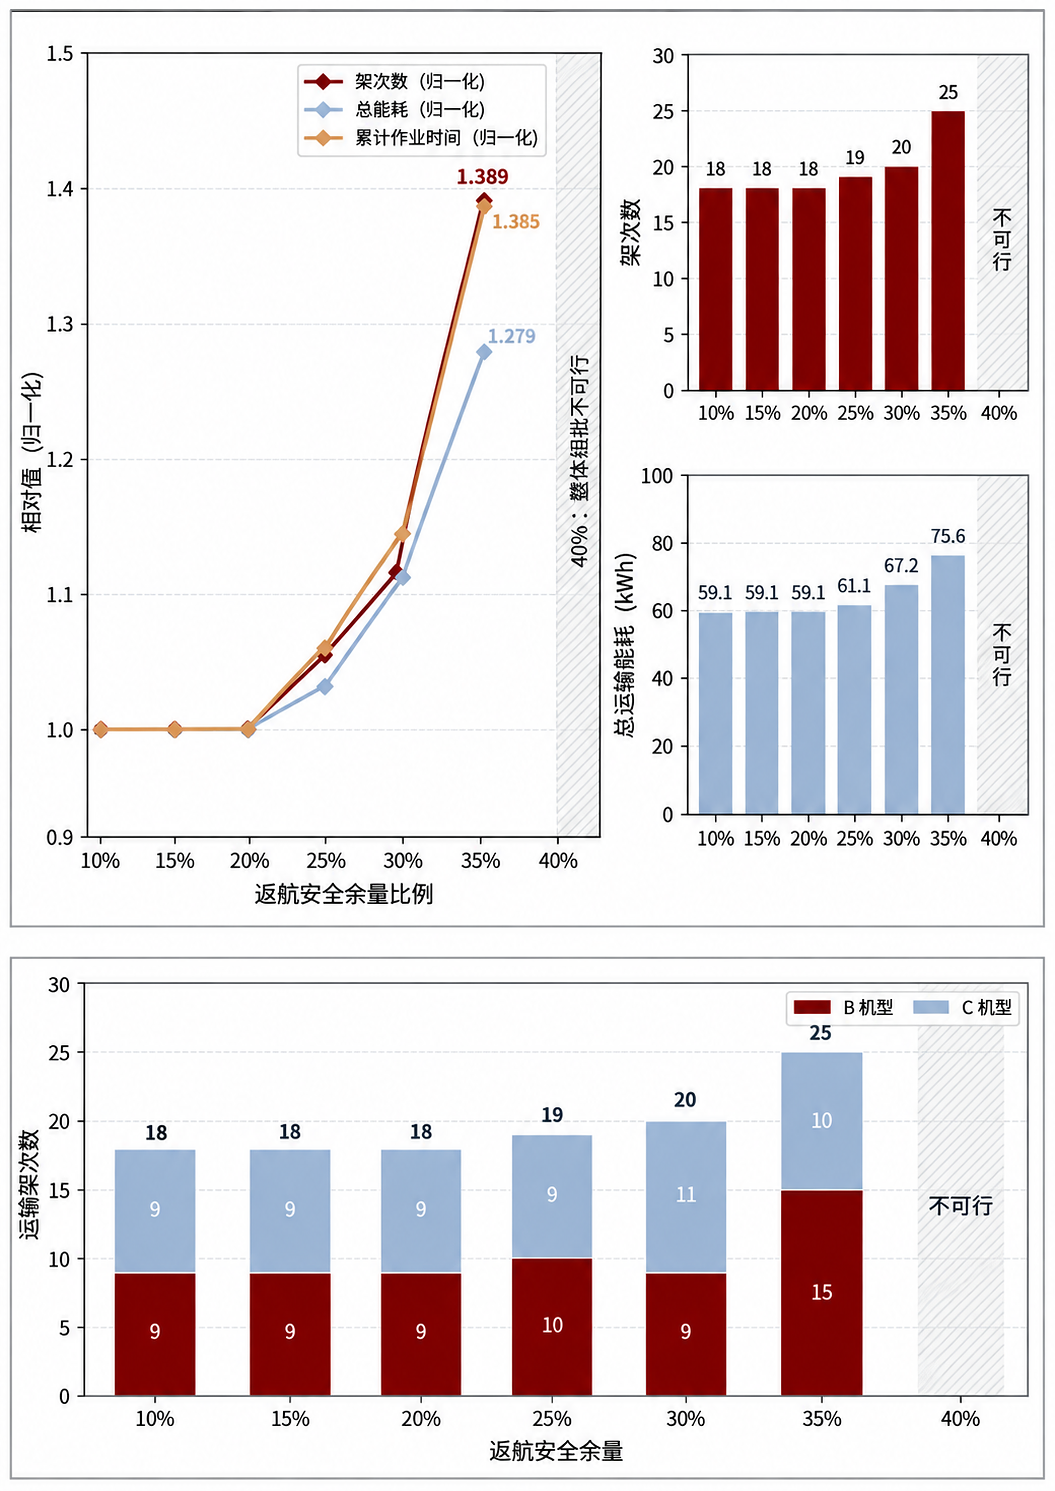
\includegraphics[width=0.8\textwidth]{figures/返航余量与组批结构、能耗、时间.png}
  \caption{返航安全余量对组批结构、总能耗和累计作业时间的影响}
  \label{fig:q1-reserve-sensitivity}
\end{figure}

图~\ref{fig:q1-reserve-sensitivity}的左上子图以20\%余量方案为基准，对架次数、总能耗和累计作业时间进行归一化；右侧给出架次数和总能耗的绝对值，底部给出B、C两型的架次数构成。10\%--20\%范围内，连续安全载荷虽已发生变化，但尚未使当前最优货箱组合失效，因此方案均保持18架次、B/C各9架次。余量提高至25\%、30\%和35\%后，总架次数分别升至19、20和25，机型构成也随之调整；35\%时总能耗和累计作业时间相对20\%方案分别增加约27.9\%和38.5\%。40\%这一测试水平下整体组批不可行，因此图中不定义相应的能耗和时间指标。

该结果反映出不可拆货箱带来的阈值效应：连续安全载荷随余量提高而平滑下降，但组批方案只在某个原有货箱组合失去可行性时才发生离散跳变。需要注意，40\%不可行仅对应本次测试点，不能据此把40\%解释为精确的可行性临界值。

为进一步解释这一变化，选取S008比较三类机型的安全载荷随返航余量的变化，如图~\ref{fig:q1-s008-sensitivity}所示。

\begin{figure}[htbp!]
  \centering
  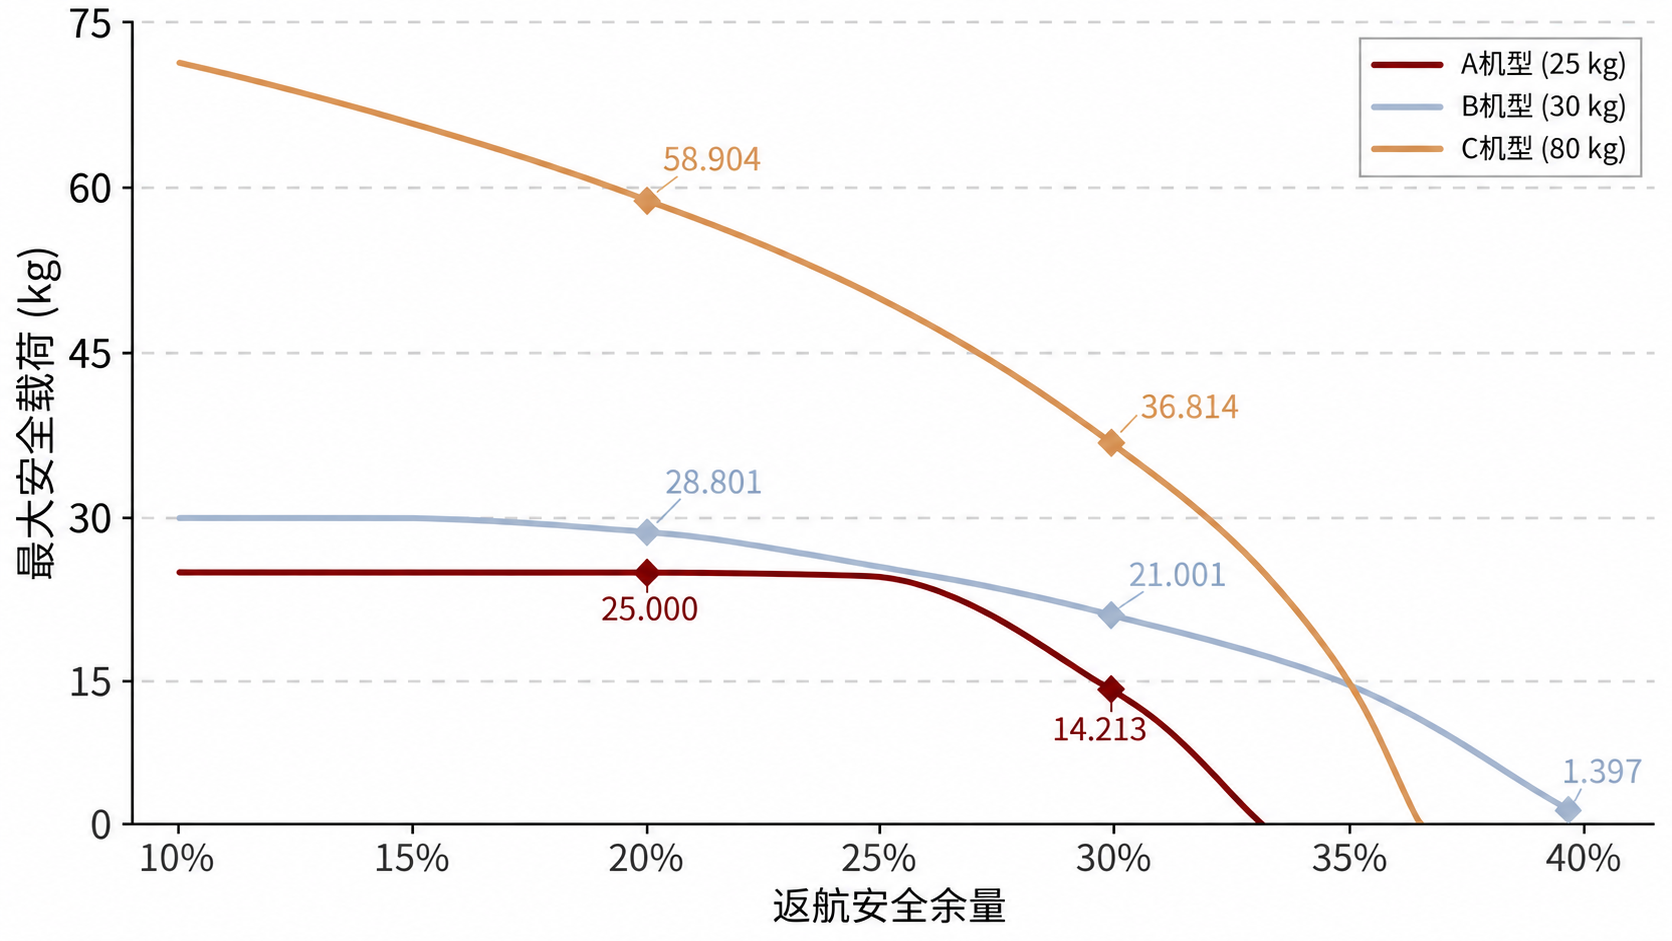
\includegraphics[width=0.8\textwidth]{figures/s800.png}
  \caption{典型困难服务区S008的最大安全载荷随返航余量变化}
  \label{fig:q1-s008-sensitivity}
\end{figure}

图~\ref{fig:q1-s008-sensitivity}中的离散实验点来自7组返航余量计算。20\%余量下，A、B、C三型的最大安全载荷分别为25.000、28.801和58.904\,kg；30\%时分别降至14.213、21.001和36.814\,kg；35\%时A型已无法满足空载安全往返要求，C型仅剩15.683\,kg；40\%时A、C两型均不可达，B型仅能携带约1.397\,kg。由此可见，S008的连续运输能力随安全余量收紧显著下降，并最终触发组批架次数的增加和整体不可行。

\subsubsection{方案可行性与求解精确性检验}
为避免仅依赖主求解程序，本文从物理约束、数值计算和离散优化三个层面进行复核。

首先，对18个最终架次逐一回代质量、体积和能量约束，并核对80个货箱的唯一覆盖关系。关键极值见表~\ref{tab:q1-feasibility-check}。

\begin{table}[htbp!]
  \centering
  \small
  \setlength{\tabcolsep}{5pt}
  \renewcommand{\arraystretch}{1.15}
  \caption{最终组批方案的物理约束核验摘要}
  \label{tab:q1-feasibility-check}
  \begin{tabular*}{0.94\linewidth}{@{\extracolsep{\fill}}lccc@{}}
    \toprule
    核验指标 & 最不利结果 & 对应架次 & 判定 \\
    \midrule
    额定载质量利用率 & 97.5\% & Q1-002 & $<100\%$，通过 \\
    装载体积利用率 & 92.4\% & Q1-001 & $<100\%$，通过 \\
    安全能量预算利用率 & 96.140\% & Q1-007 & $<100\%$，通过 \\
    最低返航SOC & 23.088\% & Q1-007 & $>20\%$，通过 \\
    货箱覆盖 & 80/80，且无重复 & 全部架次 & 通过 \\
    \bottomrule
  \end{tabular*}
\end{table}

表~\ref{tab:q1-feasibility-check}表明，18个架次均满足三类物理约束。其中Q1-007的安全能量预算利用率最高，为96.140\%，其返航SOC为23.088\%，仍高于20\%下限；因此当前方案中不存在隐藏的能量违约。

其次，对7个余量水平、3种机型和15个服务区形成的315条安全载荷记录采用独立公式实现重新计算。主程序使用Brent法求根，独立核验使用二分法；有限数值的最大绝对差为 $3.49\times10^{-11}$\,kg，8条不可达记录也完全一致。对120条无向航段的DEM最高高程进行约1\,m间距的独立密集采样复核，未发现不一致。

最后，以相同可行组批模式建立0--1整数规划，对15个服务区分别验证最少架次数及固定该架次数后的最小能耗，结果见表~\ref{tab:q1-validation}。

\begin{table}[htbp!]
  \centering
  \small
  \setlength{\tabcolsep}{5pt}
  \renewcommand{\arraystretch}{1.15}
  \caption{动态规划与0--1整数规划交叉验证结果}
  \label{tab:q1-validation}
  \begin{tabular*}{0.92\linewidth}{@{\extracolsep{\fill}}crrcc@{}}
    \toprule
    服务区 & 最少架次数 & \shortstack{对应能耗\\ /$\mathrm{kWh}$} & MILP gap & 一致性 \\
    \midrule
    S001 & 2 & 5.9134 & 0.0 & 通过 \\
    S002 & 2 & 8.4346 & 0.0 & 通过 \\
    S003 & 2 & 8.5449 & 0.0 & 通过 \\
    S004 & 1 & 6.1529 & 0.0 & 通过 \\
    S005 & 1 & 4.2222 & 0.0 & 通过 \\
    S006 & 1 & 2.5980 & 0.0 & 通过 \\
    S007 & 1 & 3.4109 & 0.0 & 通过 \\
    S008 & 1 & 5.8360 & 0.0 & 通过 \\
    S009 & 1 & 2.0962 & 0.0 & 通过 \\
    S010 & 1 & 1.8232 & 0.0 & 通过 \\
    S011 & 1 & 1.0740 & 0.0 & 通过 \\
    S012 & 1 & 2.7524 & 0.0 & 通过 \\
    S013 & 1 & 1.8248 & 0.0 & 通过 \\
    S014 & 1 & 2.1404 & 0.0 & 通过 \\
    S015 & 1 & 2.3075 & 0.0 & 通过 \\
    \bottomrule
  \end{tabular*}
\end{table}

15个服务区的MILP最优间隙均为0，最少架次数和对应最小能耗与动态规划完全一致。单个服务区枚举的可行模式数最多为201个，记忆化动态规划实际访问状态数最多为165个；本次运行记录的问题一主求解时间约0.679\,s，该数值仅用于说明本实例的计算规模。上述结果表明，所采用的状态压缩动态规划在本实例上既能保持精确性，也具有较低的计算开销。

\subsection{问题一求解结果总结与讨论}
问题一的四项要求均得到对应结果。默认20\%返航安全余量下，A型在15个服务区均可达到25\,kg额定载荷；B型仅S008降至28.801\,kg；C型在S002、S003、S004、S008和S012受到能量约束，其中S008最低，为58.904\,kg。

在货箱不可拆分、唯一分配并同时满足质量、体积和返航能量约束的条件下，80个货箱最终组成18个直接往返架次，B型和C型各9架次，总运输能耗为59.1313\,kWh，累计作业时间为9.104\,h。18个架次均通过物理约束回代，80个货箱无重复、无遗漏。

目标对照表明，若改为能耗优先，只能将总能耗降低0.165\%，却需增加1个架次，并使累计作业时间增加5.08\%；时间优先方案则与本文方案一致。因此，本实例采用“架次数--能耗--累计作业时间”的字典序具有明确的数值依据。

返航安全余量从10\%提高到20\%时，最优方案仍保持18架次；提高到25\%、30\%和35\%后，架次数分别增至19、20和25，能耗与累计作业时间同步上升；40\%测试点下整体组批不可行。该变化说明，连续安全载荷的下降会在跨越某一离散货箱组合阈值后触发组批方案跳变。上述结果为问题二引入实体无人机、共享电池和配送时限后的联合调度提供了经过验证的单架次物理可行性基础。

\FloatBarrier

\section{问题二的建模与求解}
\subsection{问题二分析}
问题一把各服务区分开组批，因而未涉及实体无人机和电池在时间上的竞争。问题二允许同一架次访问多个服务区；一条路线的箱数、访问顺序和机型一经改变，沿途载荷、送达时刻及返航电量都会随之变化。即使若干架次分别满足航程约束，同时起飞也可能超过同型运输机或共享电池的库存。因此，本问须同时决定“哪些架次执行”和“何时由哪套设备执行”。

本文把单架次的空间与物理计算放在候选路线预处理中，把货箱覆盖、时限和资源周转放在整数排程中处理。前者保留多点访问的可能性，后者使运输机与电池的占用时段能够统一比较。图~\ref{fig:q2-resources}展示最终方案的两类资源时间轴；其中浅色区间是电池返航后充电及保守预留时间，不能作为下一架次的可用时间。

本问沿用问题一的航段时间和载荷相关能耗函数，以$E_g$表示机型$g$的可用满电能量、$p_g$表示返航最低电量比例；$T_g^{\rm full}$为题给从空电至满电的充电时长。箱$b$的期望交付时刻、适用的硬截止时刻和优先系数依次记为$D_b,H_b,w_b$。后文任务开始时刻均指准备开始，实际起飞还须完成准备和装载；这一区别影响交付偏移及资源时间轴。

若机型$g_p$的候选架次$p$耗电$E_p$，其返航电量比例为$u_p=1-E_p/E_{g_p}$。将题给前90\%与后10\%电量区间的充电时间分别线性分配，得到机型$g$从任意比例$u$充至满电的时间
\begin{equation}
T_g^{\rm chg}(u)=
\begin{cases}
T_g^{\rm full}[0.65(0.90-u)/0.90+0.35],&u<0.90,\\
0.35T_g^{\rm full}(1-u)/0.10,&u\geq0.90.
\end{cases}
\label{eq:q2-charge}
\end{equation}
架次返航即释放运输机，所用电池在充满前仍占用库存；因此排程中必须分别追踪这两条时间线。

\subsection{基本约定与候选架次构造}
记$\mathcal B$为80个不可拆货箱集合，$\mathcal P$为预处理得到的候选运输架次。一个候选$p$包含货箱集合$B_p$、机型$g_p$和$n_p$个有序停靠服务区$(a_1,\ldots,a_{n_p})$，其路径为$O_{01}\to a_1\to\cdots\to a_{n_p}\to O_{01}$。同一服务区的货箱在一次停靠中交接；每个架次从满电池出发，到中心返航后才可更换或复用资源。货箱交付时刻取对应服务区卸载和交接结束时刻。

\subsubsection{逐航段载荷、时间和能源}

设$p$在航段$j$开始前尚未交付的货箱质量为$q_{pj}$，则$q_{p1}=\sum_{b\in B_p}m_b$。若第$j$站为$a_j$，离开该站后的载荷按$q_{p,j+1}=q_{pj}-\sum_{b\in B_p\cap B_{a_j}}m_b$更新；返航航段的载荷为零。因而跨区访问顺序不仅改变各箱送达时刻，也改变后续航段的能耗。

设架次$p$中第$j$个航段的起点和终点分别为$u_j$和$v_j$，其中$j=1,\ldots,n_p+1$，末段由$a_{n_p}$返回$O_{01}$。沿用问题一建立的航段飞行时间模型$t_{ij}(g)$和航段能耗模型$E_{ij}(g\mid q)$，则架次$p$的总作业时间和总能耗分别为

\begin{equation}
\begin{aligned}
d_p={}&t^{\rm prep}_{g_p}+|B_p|t^{\rm load}_{g_p}
+\sum_{j=1}^{n_p+1}t_{u_jv_j}(g_p)\\
&+\sum_{j=1}^{n_p}
\left(
t^{\rm service}_{g_p}
+|B_p\cap B_{a_j}|t^{\rm unload}_{g_p}
\right),
\\
E_p={}&\sum_{j=1}^{n_p+1}E_{u_jv_j}(g_p\mid q_{pj}).
\end{aligned}
\label{eq:q2-route-physics}
\end{equation}

对停靠序列中的第$k$个服务区$a_k$（$1\le k\le n_p$），记到达该区的航段为$u_k\to a_k$，其中$u_1=O_{01}$、$u_j=a_{j-1}$（$j>1$）；令$B_{a_j}$为目的地是$a_j$的货箱集合。交接完成才算送达，因此属于$a_k$的箱$b$有
\begin{equation}
\delta_{pb}=t^{\rm prep}_{g_p}+|B_p|t^{\rm load}_{g_p}
+\sum_{j=1}^{k}t_{u_j a_j}(g_p)
+\sum_{j=1}^{k}\left(t^{\rm service}_{g_p}
+|B_p\cap B_{a_j}|t^{\rm unload}_{g_p}\right).
\label{eq:q2-delivery-offset}
\end{equation}
式~\eqref{eq:q2-delivery-offset}不含从最后一个服务区返航的时间，而式~\eqref{eq:q2-route-physics}中的$d_p$包含返航。因此单架次可以在返回中心之前完成多个不同时间的交付。对首批保障箱，用实际交接结束时刻判断时限，不能用起飞或到站时刻替代。

候选架次只有在起飞质量、体积、逐段航迹以及
\[
E_p\le(1-p_{g_p})E_{g_p}
\]
均满足要求时才予以保留；即使立即开始准备也无法满足硬时限的候选同样剔除。这里的能量约束考察的是整个架次的返航余量，不能把每段分别可飞误当作整条路线可飞。

\subsubsection{有限候选池的构造}
候选池先纳入问题一的单区组批、每箱单独运输以及同区双箱组合，确保每个货箱至少存在基本投送选择。随后以固定随机种子进行55轮单区与55轮跨区受限组批：逐步增加货箱，对新服务区尝试不同插入位置，每条路线至多访问三个服务区；最后对已构造的货箱组合与访问顺序尝试其他可行机型。以“机型—货箱集合—访问顺序”去重，得到3988条候选，其中单区1783条、跨区2205条。完整货箱覆盖由后续式~\eqref{eq:q2-cover}保证；候选池覆盖所有箱并不意味着穷举了全部可能组批和访问顺序，因此不能从池内搜索结果推出原问题的全局最优。

\subsection{货箱覆盖、时限与共享资源模型}
\subsubsection{一次交付和时限}
令$x_p\in\{0,1\}$表示是否执行候选$p$，$s_p\in\mathbb Z_{\geq0}$为其准备开始时刻。任何货箱恰由一条选中路线交付：
\begin{equation}
\sum_{p:\,b\in B_p}x_p=1,\qquad b\in\mathcal B.
\label{eq:q2-cover}
\end{equation}
箱$b$在被选中的架次$p$中完成交接的实际时刻为$C_b=s_p+\delta_{pb}$。对具有硬截止时刻$H_b$的首批保障箱及医疗箱施加$C_b\le H_b$；题给期望时刻$D_b$用于衡量迟到，令$T_b=\max\{0,C_b-D_b\}$。当同一箱同时受到首批保障和医疗时限约束时，取较早的硬截止时刻。未设置硬截止的箱可以迟于$D_b$，但会付出加权迟到代价。
整数秒求解时，$s_p$为整数且各候选交付偏移向上取整，即$\widehat C_b=s_p+\lceil\delta_{pb}\rceil$。硬时限在求解器内写为$\widehat C_b\le\lfloor H_b\rfloor$；这样选中的排程回到连续物理时间后仍满足$C_b\le H_b$，但边界上可能排除本可行的非整数秒方案。该保守性是后文最优性结论只针对整数秒模型的原因之一。

\subsubsection{运输机与共享电池的双区间占用}
记机型$g$现有运输机数和电池数为$N_g^{\rm drone},N_g^{\rm bat}$，本题分别为A型$4/6$、B型$2/4$、C型$2/4$。运输机占用到实际返航，电池则还须经历式~\eqref{eq:q2-charge}给出的分段充电。为在整数秒排程中保守处理非整数时长，定义
\begin{equation}
\widehat d_p=\lceil d_p\rceil,\qquad
\widehat b_p=\left\lceil d_p+T_{g_p}^{\rm chg}
\left(1-\frac{E_p}{E_{g_p}}\right)\right\rceil.
\label{eq:q2-reserved-length}
\end{equation}
选择架次$p$时，运输机占用$[s_p,s_p+\widehat d_p)$，电池占用$[s_p,s_p+\widehat b_p)$。对每种机型和任意时刻$t$，两类并发数分别不得超过其库存：
\begin{align}
\sum_{p:g_p=g}x_p\mathbf 1_{[s_p,s_p+\widehat d_p)}(t)
&\le N_g^{\rm drone},\\
\sum_{p:g_p=g}x_p\mathbf 1_{[s_p,s_p+\widehat b_p)}(t)
&\le N_g^{\rm bat}.
\label{eq:q2-cumulative}
\end{align}
整数模型中两组区间分别用可选区间与累积容量约束表达。求解后再按区间不重叠原则把任务匹配至具体机号、电池号，并以未取整的物理时刻复核。此时表~\ref{tab:q2-result}中的完工时间按实际返航计算，与整数目标中的向上取整完工值略有差别。

这里把$H_b$与$D_b$分开是必要的：前者一旦违反，方案即不可行；后者只改变方案的优劣。对没有硬截止的箱不人为补造截止时刻；对两项硬要求同时适用的箱取较早时刻，也避免重复计算。半开资源区间允许上一任务的释放时刻恰好等于下一任务的开始时刻，与充电完成后立即复用电池一致。未选路线的可选区间不占用库存，因此货箱覆盖和资源容量可在同一模型内联立求解。

表~\ref{tab:q2-model-map}将候选预处理与排程求解的边界列出。航程、载荷和返航电量在生成候选时已检查，因而整数模型无须重复展开每个飞行航段；相反，同型机和电池的同时占用取决于所有已选架次的起始时刻，只能在排程层联立判断。这种划分减少了组合模型的规模，也使回代时可以分别核查“路线自身是否可飞”和“多条路线能否同时执行”。
\begin{table}[htbp]
\centering\small
\caption{两层计算中的主要变量约束与核查对象}
\label{tab:q2-model-map}
\begin{tabular}{@{}p{0.17\textwidth}p{0.36\textwidth}p{0.39\textwidth}@{}}
\toprule
层次 & 决策或计算量 & 可行性条件与作用\\
\midrule
路线预处理 & 货箱集合、机型、停靠顺序；$d_p,E_p,\delta_{pb}$ & 质量、体积、逐段载荷及返航电量；剔除即时起飞亦不满足硬时限的路线\\
整数排程 & 路线选择$x_p$、准备开始$s_p$、整数交付$\widehat C_b$ & 80箱恰好覆盖一次；硬截止时刻；运输机与电池分别满足累积容量\\
物理回代 & 实际交付$C_b$、返航时刻与电池就绪时刻 & 恢复未取整航段值，逐箱、逐资源检查最终排程\\
\bottomrule
\end{tabular}
\end{table}

\subsection{优化目标与求解方法}
\subsubsection{整数化加权目标}
本问同时关心送达及时性、最后返航时间、能耗和架次数。为使求解器能够直接比较不同候选路线，采用代码中\texttt{balanced}配置的单一整数目标。设$\widehat C_b=s_p+\lceil\delta_{pb}\rceil$、$\widehat T_b=\max(0,\widehat C_b-D_b)$，并令$\widehat M=\max_{p:x_p=1}(s_p+\widehat d_p)$，则
\begin{equation}
\min\;100\widehat M
+\sum_{b\in\mathcal B}w_b\bigl(\widehat C_b+100\widehat T_b\bigr)
+\sum_{p\in\mathcal P}x_p\left[10\,\operatorname{round}(1000E_p)+10000\right].
\label{eq:q2-objective}
\end{equation}
这里$w_b$是题给优先系数。式~\eqref{eq:q2-objective}是加权和，并非严格字典序；报告“迟到为零”是求得排程的事实，不应理解为目标函数强制零迟到。能耗项以Wh取整，所有系数均为本次计算采用的权重，不把它们解释成真实货币成本。

式中的$\widehat M$由已选架次的整数返航时刻最大值等式实现，$\widehat T_b$由非负变量及$\widehat T_b\geq\widehat C_b-D_b$实现。迟到项系数为正，故最优时$\widehat T_b$取可行最小值。求解器中的秒级向上取整用于避免低估资源占用，正式结果仍以未取整的航段物理量回代。

\subsubsection{候选池求解与固定路线重排}
CP-SAT先在有限候选池内联合选择路线和开始时刻，原始目标值为4290638。随后固定24条选中路线和货箱分配，只重排整数秒开始时刻及两类容量资源。新目标值为4281382，减少9256（约0.216\%）。

固定路线子问题的求解状态为\texttt{OPTIMAL}，目标值与下界同为4281382。

表~\ref{tab:q2-objective-parts}按式~\eqref{eq:q2-objective}拆开重排前后的目标值。路线和货箱分配未变，故架次数与能耗项不变；联合返航完工项也相同。9256的改善全部来自货箱加权交付时刻提前，而不是架次数或能耗减少。这个拆解同时检验了目标函数计算与正式逐箱交付表的一致性。
\begin{table}[htbp]
\centering\small
\renewcommand{\arraystretch}{1.15}
\caption{固定路线重排前后目标值分项}
\label{tab:q2-objective-parts}
\begin{tabularx}{\textwidth}{@{}l *{3}{>{\raggedleft\arraybackslash}X} @{}}
\toprule
分项 & 原排程 & 重排后 & 改变量\\
\midrule
联合完工项 & 699800 & 699800 & 0\\
加权交付项 & 2655038 & 2645782 & $-9256$\\
加权迟到项 & 0 & 0 & 0\\
能耗项 & 695800 & 695800 & 0\\
架次数项 & 240000 & 240000 & 0\\
\midrule
总目标值 & 4290638 & 4281382 & $-9256$\\
\bottomrule
\end{tabularx}
\end{table}

为考察更换组批和访问顺序的可能改进，还进行了20轮大邻域重建：每轮移出5--9条当前路线，补入相关替代路线和部分成对合并路线，给CP-SAT 8\,s搜索时间，随机种子为20260923。20轮均未接受更优解；因此，本次已实现的目标值改善来自前述固定路线重排，不能归因于大邻域搜索。“固定路线最优”也仅针对这24条路线、整数秒开始时刻和给定资源模型，不证明3988条候选池或全部可行路线上的全局最优。

\subsection{计算结果与分析}
\subsubsection{运输任务与机型分工}
表~\ref{tab:q2-result}给出正式方案。24个架次交付80箱，A、B、C型分别执行10、8、6架次；其中C型6架次承运39箱，体现大载重机型的组批能力。仅两条已选架次访问两个服务区：\texttt{Q2-009}沿$S009\to S012$运行，\texttt{Q2-020}沿$S011\to S014$运行。候选池虽包含大量跨区路线，但本次求得的排程主要采用单区组批；跨区路线的价值取决于具体货箱、顺序和时限，不能由已选比例推断其普遍优劣。

作为候选策略对照，把问题一的18条既定组批路线原样施加问题二的时限和双资源约束，模型返回不可行。这表明原组批不能直接沿用，并不证明问题二至少需要19架次。仅从1783条单区候选中求得的可行排程为26架次、71.599\,kWh；允许2205条跨区候选参加选择后，找到24架次、69.580\,kWh的方案，随后固定这24条路线优化时序。表~\ref{tab:q2-strategy}按未取整的物理时刻与能耗比较这些已求得的方案，其中平均交付时刻按货箱优先系数加权。两种候选策略均受候选池与搜索时间限制，表中的2架次差额只描述本次所得方案，不能据此认定跨区运输必然节省2架次。
\begin{table}[htbp]
\centering
\small
\renewcommand{\arraystretch}{1.15}

\caption{候选策略的运输结果}
\label{tab:q2-strategy}

\begin{tabularx}{\textwidth}{
    @{}l
    *{4}{>{\raggedleft\arraybackslash}X}
    @{}
}
\toprule
方案 & 架次 & 跨区架次 & 电耗/kWh & 加权平均交付/s\\
\midrule
仅单区候选     & 26 & 0 & 71.599 & 2781.010\\
跨区候选原排程 & 24 & 2 & 69.580 & 2776.663\\
固定路线重排后 & 24 & 2 & 69.580 & 2766.981\\
\bottomrule
\end{tabularx}

\end{table}

\begin{table}[htbp]
\centering\small
\renewcommand{\arraystretch}{1.15}
\caption{正式运输方案汇总}
\label{tab:q2-result}

\begin{tabularx}{\textwidth}{
    @{}l
    *{3}{>{\raggedleft\arraybackslash}X}
    @{}
}
\toprule
指标 & A型 & B型 & C型\\
\midrule
运输架次       & 10     & 8      & 6\\
交付货箱数     & 20     & 21     & 39\\
运输能耗/kWh   & 27.125 & 17.716 & 24.740\\
\midrule
\multicolumn{3}{@{}l}{全部货箱/全部架次}   & 80 / 24\\
\multicolumn{3}{@{}l}{加权迟到/迟到箱数}   & 0 / 0\\
\multicolumn{3}{@{}l}{运输返航完工时间/s}   & 6997.523\\
\multicolumn{3}{@{}l}{总运输能耗/kWh}       & 69.580\\
\multicolumn{3}{@{}l}{最小返航电量比例}     & 23.088\%\\
\multicolumn{3}{@{}l}{最小硬时限剩余时间/s} & 220.525\\
\bottomrule
\end{tabularx}
\par\footnotesize 注：各机型能耗独立保留三位小数，显示值之和与按原始数据计算的总量相差0.001\,kWh。

\end{table}
图~\ref{fig:q2-resources}按具体机号和电池号绘制排程：上半部分为运输机占用，下半部分为电池占用；实色从准备开始延续到返航，浅色表示返航后的充电及保守预留。前8个架次在$t=0$同时开始准备，之后的任务由已返航运输机及可用电池接续执行。由正式区间直接求得A、B、C型运输机峰值分别为$4/2/2$架，共享电池峰值分别为$6/4/4$块，恰与各型现有库存相等。只看运输机的空闲而忽略电池浅色区间，会高估可同时出动的能力；本图也给出了同型电池在不同实体机之间周转的实际安排。
\begin{figure}[htbp]
\centering

\includegraphics[width=0.8\textwidth]{figures/result_q2_resources_cn.pdf}
\caption{运输机与共享电池占用时序}
\label{fig:q2-resources}
\end{figure}

\subsubsection{送达时效与安全余量}
80箱均在期望时刻前交付，加权迟到为零；加权平均交付时刻为2766.981\,s。图~\ref{fig:q2-slack}按服务区排列有硬截止的货箱：横轴为余量$(H_b-C_b)/60$（min），点表示逐箱结果，横线连接同区最小与最大余量。所有点均位于零线右侧；空心圆标出的饮用水箱\texttt{S012-\allowbreak{}WAT-01}最紧，仍提前220.525\,s。若临时延迟相关架次，应首先复查此箱的硬时限。所有架次最小返航电量比例为23.088\%。
\begin{figure}[htbp]
\centering
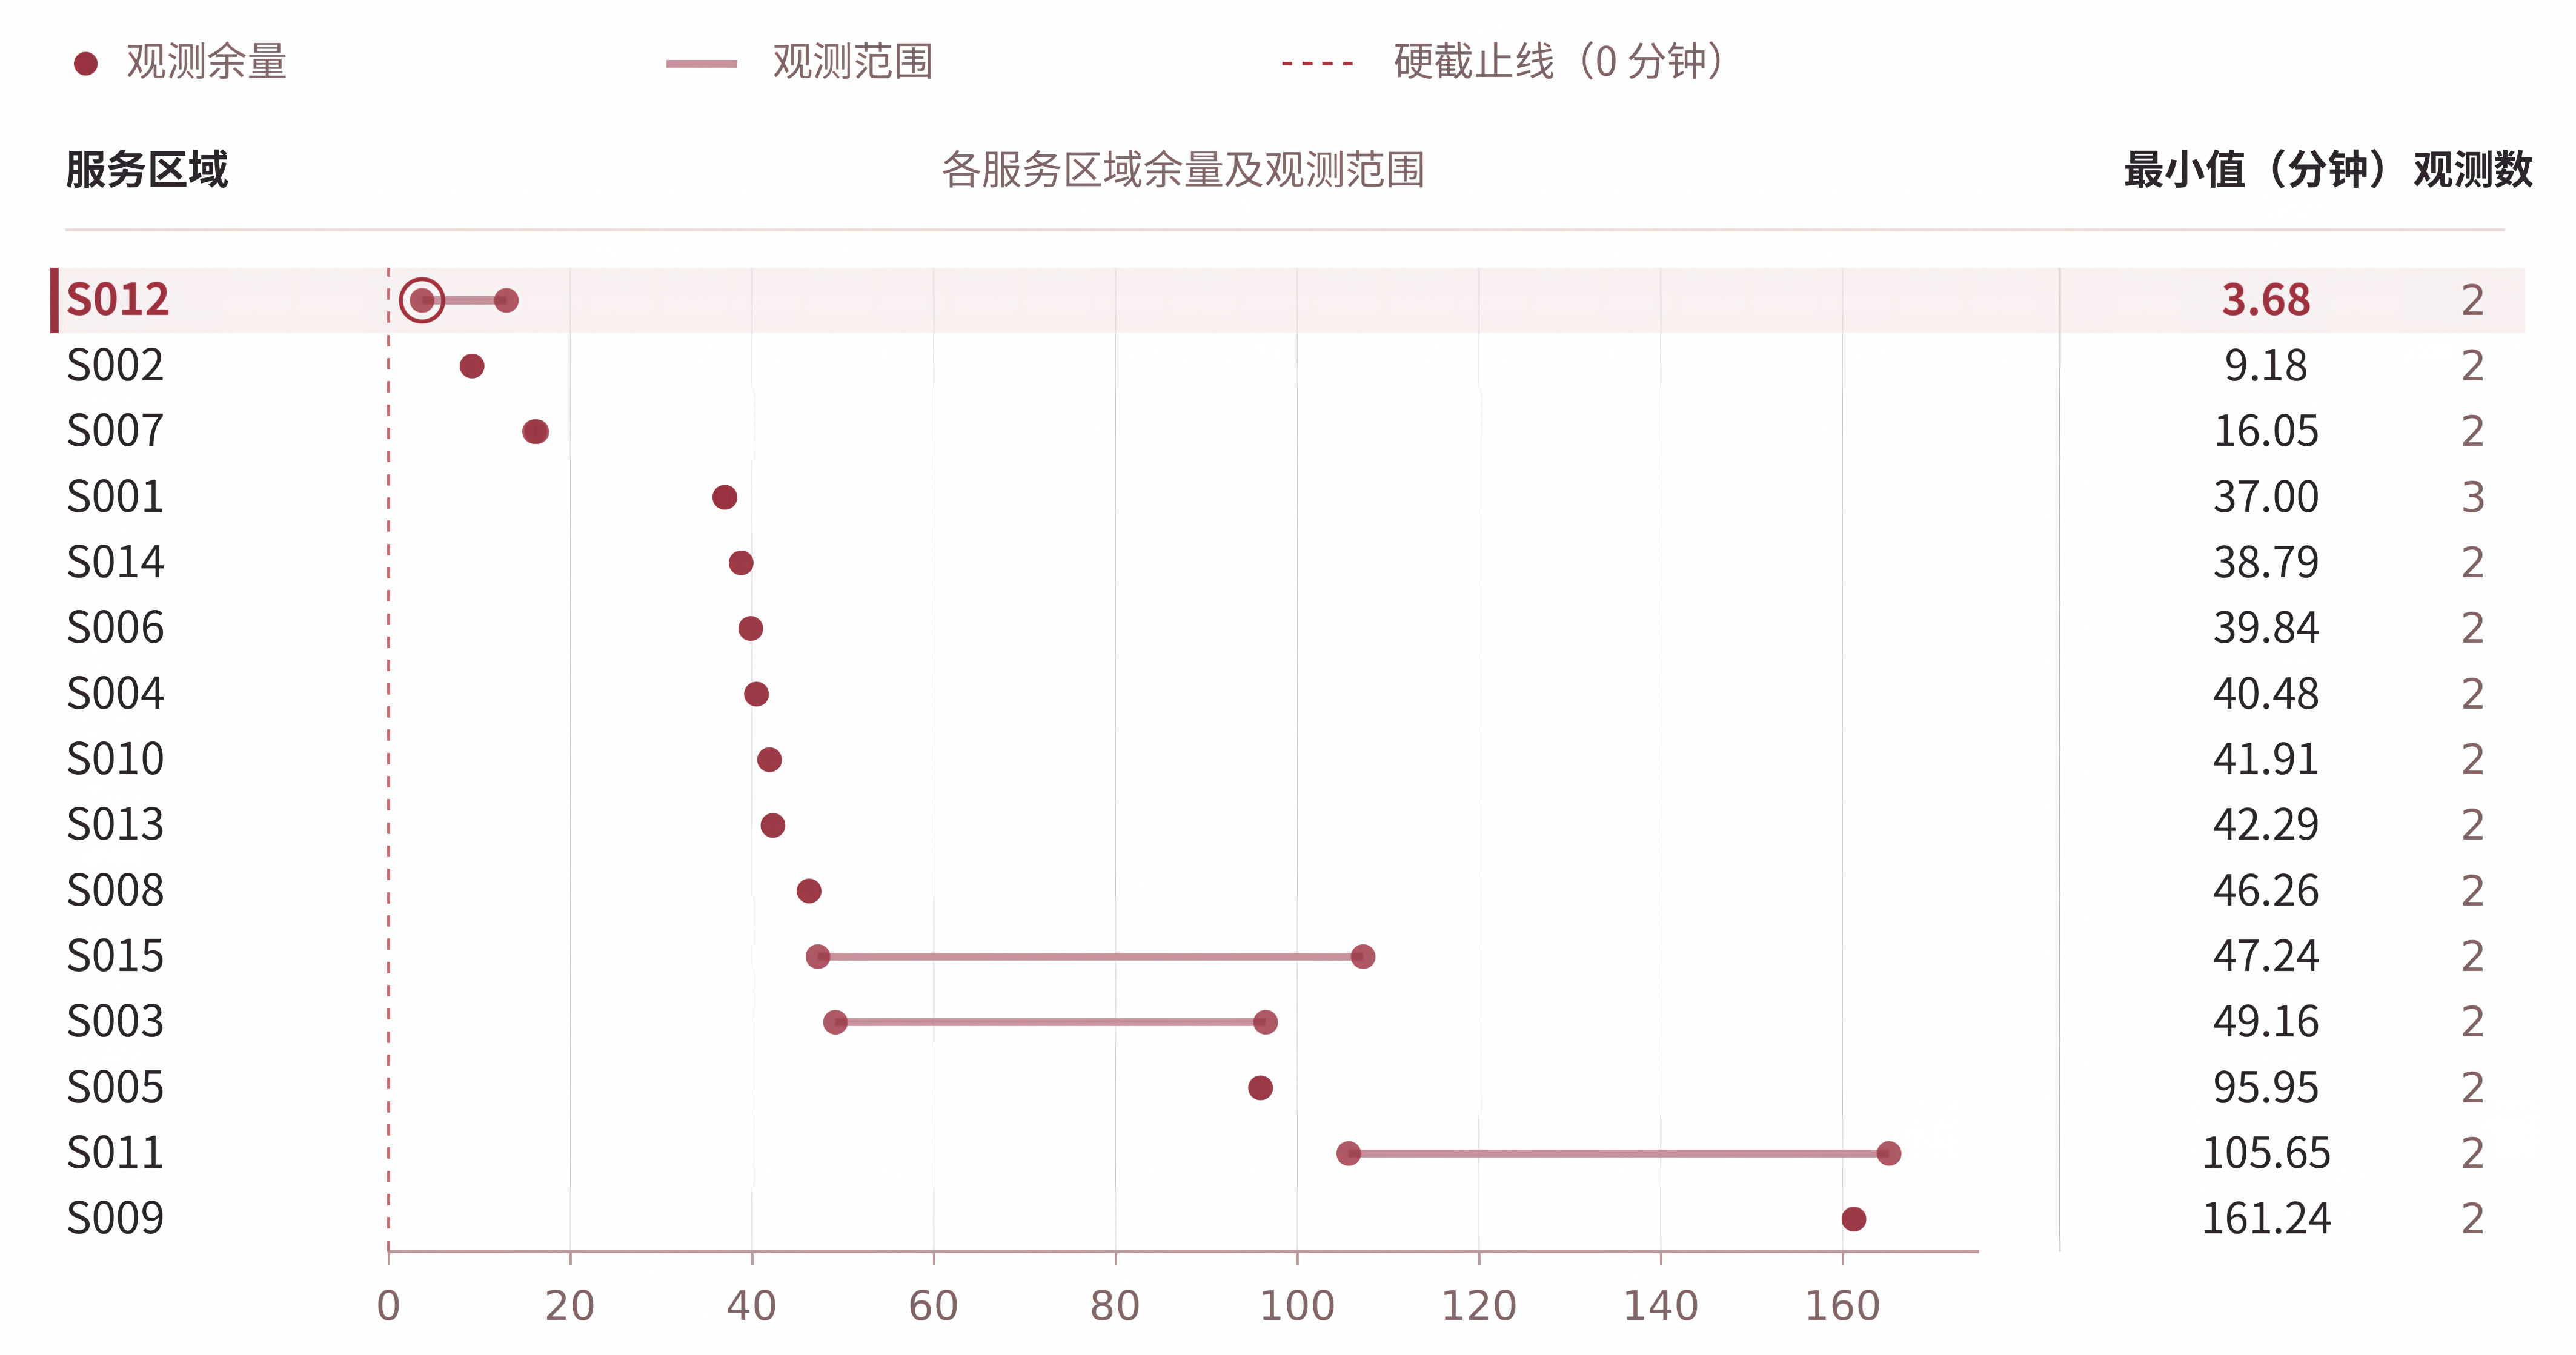
\includegraphics[width=0.8\textwidth]{figures/result_q2_hard_deadline_margin(1).png}
\caption{硬截止货箱的交付余量}
\label{fig:q2-slack}
\end{figure}

\subsection{正确性与最优性范围检验}
正式结果保存了逐架次、逐箱、逐航段和电池周转记录。逐箱核对80个箱的唯一交付、交付时刻与对应服务区；逐航段重新累加飞行时间和载荷相关能耗，检查起飞质量、体积及返航电量；再将每条路线配给具体机号、电池号，检查同一资源的占用区间是否相交。表~\ref{tab:q2-audit}列出相互独立的核查对象与结果。硬时限和期望时刻仍按各自定义分别计算，不能用“迟到箱数为零”代替硬约束验证。
\begin{table}[htbp]
\centering\small
\caption{正式排程的逐项回代核查}
\label{tab:q2-audit}
\begin{tabular}{@{}p{0.26\textwidth}p{0.47\textwidth}r@{}}
\toprule
核查对象 & 回代依据 & 结果\\
\midrule
不可拆货箱 & 逐箱记录与80箱清单逐一匹配 & 80箱唯一交付\\
硬截止时刻 & 对适用的箱计算$H_b-C_b$ & 最小余量220.525\,s\\
返航电量 & 逐航段电耗除以机型可用电能 & 最小23.088\%\\
运输机与电池 & 具体设备占用、返航与充满区间 & 冲突0次\\
固定路线整数排程 & 目标值与该子问题下界 & 均为4281382\\
\bottomrule
\end{tabular}
\end{table}

最后一行的最优证书只证明已选24条路线在给定整数秒模型下的排程最优。候选生成没有穷举所有货箱组合，原候选池求解也没有匹配全局上下界；20轮大邻域搜索未接受新解只能说明这些受限邻域没有找到改进。故问题二的完整结果应称为物理与资源约束均已验证的可行调度。第三问将加入连续通信约束，并允许调整部分运输时刻。

\subsection{问题二求解结果总结与讨论}
问题二把候选路线的逐段物理计算与多架次的双资源排程联立，得到24架次完成80箱交付、全部期望时刻和硬截止时刻均满足的运输方案。运输机和电池的峰值均达到现有库存，说明充电周转不能从排程中省去。固定已选路线后的整数秒时序具有最优性证书，但候选池未穷尽所有路线；因而该方案可作为第三问加入通信保障的已验证运输基线，而非原始问题的全局最优解。


\section{问题三的建模与求解}
\subsection{问题三分析}
问题二的24架次排程满足运输与电池周转约束，却没有检查飞行过程中能否持续与固定网关$G_{01}$通信。山区遮挡使“起飞点、服务区两端可连通”不能推出整条航迹可连通；中继又占用两架中继机和六个能源组件，其建链、悬停及充电会反过来限制运输任务开始时刻。本问因而在已有货箱分配的基础上联动调整运输时序、中继位置和服务窗口，要求每一条运输轨迹的全部需通信时段都存在有效双向链路。

初始第二问排程的直连失效比例在不同架次间差异明显，见图~\ref{fig:q3-direct-gap}。横轴为24条运输架次，纵轴为每条轨迹20\,s采样点中无法直连网关的比例；该比例只用于定位覆盖缺口，并非最终连续通信证明。中继位置若只为一个架次选择，可能产生大量短窗口；若能覆盖多条轨迹，就有机会减少中继起降和组件占用。因此，求解中把覆盖能力与任务时序同时考虑。
\begin{figure}[htbp]
\centering

\includegraphics[width=0.8\textwidth]{figures/raw_q3_q2_direct_outages.pdf}
\caption{问题二架次的网关直连缺口}
\label{fig:q3-direct-gap}
\end{figure}

\subsection{通信链路与连续覆盖模型}
通信要求作用于运输机需要保持联络的实际轨迹时间，而非仅作用于服务区或航段端点。将爬升、巡航、下降、交接及返航拆成分段轨迹；中继机到达悬停点并完成建链后才成为可用节点，返航途中不再提供覆盖。这样，通信可行性成为时间与空间同时成立的约束。
\subsubsection{双向链路预算}
对端点$a,b$，由发射功率、收发增益、系统损耗和接收灵敏度计算两个方向的允许路径损耗，并取较小值作为双向门槛。将题给8\,dB通信裕量加入各接收灵敏度，定义有效接收门槛$P_{{\rm th},i}=P_{{\rm sens},i}+8\,\mathrm{dB}$，则
\begin{equation}
L^{\max}_{a\leftrightarrow b}
=\min\!\left\{
P_a+G_a^t+G_b^r-L_{\rm sys}-P_{{\rm th},b},\;
P_b+G_b^t+G_a^r-L_{\rm sys}-P_{{\rm th},a}
\right\}.
\label{eq:q3-budget}
\end{equation}
式中发射功率与接收门槛以dBm计，天线增益以dBi计，系统损耗与路径损耗以dB计。给定时刻$t$两端点三维距离$D_{ab}(t)$（km）、工作频率$f$（MHz），用DEM判定视线是否被地形遮挡，记遮挡指示量为$z_{ab}(t)$，则
\begin{equation}
L_{ab}(t)=32.45+20\log_{10}f+20\log_{10}D_{ab}(t)
+L_{\rm obs}z_{ab}(t),\qquad
A_{ab}(t)=\mathbf1\!\left\{L_{ab}(t)\le L^{\max}_{a\leftrightarrow b}\right\}.
\label{eq:q3-link}
\end{equation}
这里$L_{\rm obs}$是题给遮挡附加损耗。运输机位置按准备后爬升、水平巡航、下降和服务区交接阶段分段计算，而非把整条路线视为一根静态直线。

\subsubsection{直连或单中继两跳保障}
记运输机$p$的通信需求时间集合为$\mathcal T_p$，并以$G_{01}$表示固定网关。若中继任务$r$已完成建链并处于悬停服务窗口，令$I_r(t)=1$；否则为0。对所有$p$及$t\in\mathcal T_p$，要求
\begin{equation}
A_{pG_{01}}(t)=1
\quad\text{或}\quad
\exists r:\ I_r(t)A_{pr}(t)A_{rG_{01}}(t)=1.
\label{eq:q3-cover}
\end{equation}
因此，两跳链路必须在\emph{同一时刻}同时成立，不能分别用不同时刻的可达性代替。模型只使用固定网关直连或“运输机—中继—网关”两跳，不引入多中继转发。题目没有给出单架中继的并发接入上限；在这一数据边界下，同一中继服务窗可同时保障多架运输机。

式~\eqref{eq:q3-cover}等价于对每个$t\in\mathcal T_p$要求至少有一个完整的通信提供者。提供者可以随时间切换，不必强迫一条运输路线始终依赖同一架中继，但切换处也必须有可用链路。只在固定步长的样点上检查，无法排除两样点之间的短暂遮挡；后续连续证书专门处理这一缺口。

\subsection{中继任务与能源资源模型}
中继并非可随意放置的静态覆盖点，而是一条从中心出发、建立回传链路、悬停服务、再返回中心的完整架次。候选点只是搜索空间；决定采用某点时，服务开始、结束、机号和能源组件仍需与运输任务共同排程。长服务窗有利于共享保障，却会增加悬停电耗并延后同一中继机或组件的下次可用时刻。
\subsubsection{候选悬停点与预筛}
候选点以服务区、中心至服务区航线上的四分点和中点及服务区附近点为基础，并在部分位置枚举不同离地高度。每个位置均由DEM取得地面高程，悬停高度不超过题给上限。候选点需同时满足中继至网关的双向回传链路、往返飞行能量和返航余量。对每条运输轨迹上的直连缺口，预计算可由哪些候选点接入。图~\ref{fig:q3-sites}展示全高度候选中覆盖20\,s初始失联样点最多的15处位置；各柱是单独放置该点时的覆盖数，彼此可以重叠，不能相加为总覆盖数。该图用于筛选位置，不作为连续通信可行性的证据。
\begin{figure}[htbp]
\centering

\includegraphics[width=0.8\textwidth]{figures/process_q3_candidate_coverage.pdf}
\caption{候选中继点的覆盖能力}
\label{fig:q3-sites}
\end{figure}

候选覆盖采用粗轨迹采样，目的是淘汰明显无效的位置，而非证明正式方案。束搜索采用候选位置的若干高度层，先检查回传和往返飞行余量，再按10\,s网格记录运输机与候选点的可达关系。若某点能覆盖多条路线的直连缺口，可通过延长悬停窗复用一次中继；若所需窗口过长或能耗超限，必须拆分架次或换点。

\subsubsection{一次中继架次的时间与电量}
一条中继架次从$O_{01}$起飞，经历准备、往程、建链、悬停服务、返程和周转。设候选点为$k_r$，建链后服务窗口为$[\sigma_r,\tau_r]$，则其电耗写为
\begin{equation}
E_r^{\rm relay}=E_r^{\rm flight}
+\frac{P_{\rm hover}+P_{\rm comm}}{3600}
\bigl(T_{\rm link}+\tau_r-\sigma_r\bigr).
\label{eq:q3-relay-energy}
\end{equation}
$E_r^{\rm flight}$由往返水平飞行功率和爬升势能共同计算；$P_{\rm hover},P_{\rm comm}$以kW计，式中时间以s计，因此除以3600后得到kWh。服务项含建链时间，避免漏计建链期间的悬停与通信耗电。中继电池返航后须保有规定比例电量。两架实体中继机的任务区间加上周转时间不得重叠；六个能源组件在其所执行任务返航并完成分段充电前不得复用。可行候选服务窗还须覆盖需要它的运输机失联时段，并在窗口两端留出预设时间缓冲。

服务窗$[\sigma_r,\tau_r]$只是实际任务的一部分。中继机占用从准备开始延续到返航及规定周转结束；组件占用则延续到返航充满，二者释放时刻通常不同。式~\eqref{eq:q3-relay-energy}中的服务时长增加，会同时推高电耗与组件充电时间，因此不能仅根据覆盖点的几何可见性决定中继数量。

具体地，令$\ell_r$为中继任务开始准备的时刻，$e_r$为返航时刻，$T^{\rm chg}_r$为根据返航电量计算的组件充电时间。中继机和能源组件分别占用半开区间
\begin{equation}
I_r^{\rm relay}=[\ell_r,e_r+300),\qquad
I_r^{\rm component}=[\ell_r,e_r+T^{\rm chg}_r).
\label{eq:q3-resource-interval}
\end{equation}
300\,s是题给的中继机返航周转时间。对同一机号和同一组件号，式~\eqref{eq:q3-resource-interval}中的相应区间不得相交；若不预先指定编号，则任意时刻的并发数分别不得超过2架中继机和6个能源组件。两种资源的释放顺序未必相同，例如中继机完成周转后可换用其他已就绪组件再次出动。实际排程同时检查这两类区间，以及中继往返飞行、建链和服务窗之间的先后关系。

\subsection{联合求解与时间细化}
若在连续时间内直接联立优化24条运输路线的时序、全部中继位置及服务窗，变量耦合很强。本文采用“粗网格生成候选—有限宽度联合排程—实例时间细化—精确回代与连续证明”的分层流程。粗网格只用于搜索，最终可行性由原始DEM、完整轨迹及时间区间证书决定。
表~\ref{tab:q3-fidelity}说明各阶段的时间分辨率和判定职责。候选点展示图~\ref{fig:q3-sites}仅使用全高度候选、20\,s初始运输轨迹样点；实际束搜索重新生成0.5、0.75和1倍高度的候选位置，并用10\,s轨迹网格建立覆盖关系。两者服务于不同步骤，不能把图中的覆盖数量当作最终服务时长或链路证明。
\begin{table}[htbp]
\centering\small
\caption{分层计算与验证口径}
\label{tab:q3-fidelity}
\begin{tabular}{@{}p{0.20\textwidth}p{0.26\textwidth}p{0.46\textwidth}@{}}
\toprule
阶段 & 位置及时间处理 & 可支持的结论\\
\midrule
候选点展示 & 全高度位置，20\,s样点 & 比较初始失联样点的候选覆盖数，用于解释选点\\
束搜索 & 三层高度，10\,s轨迹网格 & 筛选服务窗与运输时序，形成待严格验证的候选\\
事件采样回代 & 完整轨迹、最大间隔1\,s，增补服务窗边界 & 检出样点处的失联及物理、时间、资源违反\\
连续区间证书 & 阶段端点起始、最长30\,s初分，未决时二分 & 在DEM与链路模型内证明所有需求时刻都有可用提供者\\
\bottomrule
\end{tabular}
\end{table}
\subsubsection{搜索状态与排序}
以问题二的24个架次和原有货箱分配为输入。为使具有3600\,s硬截止时刻的医疗箱\texttt{S012-MED-01}先交接，跨区架次\texttt{Q2-009}的访问顺序由$S009\to S012$调整为$S012\to S009$，并重新计算逐段载荷、航时、能耗、交付偏移和电池就绪时刻。表~\ref{tab:q3-order}比较的是从任务准备开始到交付的偏移，剔除了两问任务开始时刻不同的影响。前往$S012$的交付偏移缩短295.234\,s，但$S009$的食品箱延后715.711\,s，路线能耗增加0.040388\,kWh；因此倒序不是无代价的改进。除此之外，搜索保留原有货箱分配与机型，主要调整任务时序和中继服务窗。
\begin{table}[htbp]
\centering\small
\renewcommand{\arraystretch}{1.15}
\caption{架次Q2-009的访问顺序比较}
\label{tab:q3-order}

\begin{tabularx}{\textwidth}{
    @{}
    >{\raggedright\arraybackslash}p{0.32\textwidth}
    >{\raggedleft\arraybackslash}X
    >{\raggedleft\arraybackslash}X
    >{\raggedleft\arraybackslash}X
    @{}
}
\toprule
货箱 & 原顺序偏移/s & 倒序偏移/s & 变化/s\\
\midrule
\texttt{S012-MED-01} & 1599.709 & 1304.475 & $-295.234$\\
\texttt{S009-FOD-01} & 1095.897 & 1811.608 & $+715.711$\\
\bottomrule
\end{tabularx}

\end{table}

先用10\,s网格标记各运输轨迹的网关直连缺口及候选中继点的两跳覆盖关系。问题二已选24个架次的承运货箱集合、机型及具体运输机、电池编号保持不变，只有上段所述\texttt{Q2-009}访问顺序改变；前8个架次固定在$t=0$同时开始准备，并据其直连缺口枚举初始中继点对。每个状态记录已排和未排架次、设备就绪时刻及中继任务的点位与服务窗。扩展待排架次时，依次尝试直连、复用或延长已有中继窗以及新建中继任务，并检查硬时限、能量和资源约束。排序同时考虑已发生迟到、未来紧急路线的最早可能迟到以及候选点稀缺程度；对同一初始点对及新中继点限制近似重复状态，每层最多保留160个。束宽和上述固定决策限制了搜索空间，算法不提供全局最优界。

本次实例枚举78组初始中继点对，形成79个初始搜索状态；随后对余下16条运输路线逐层扩展，累计生成37275个子状态，搜索耗时47.226\,s。表~\ref{tab:q3-search-flow}把每一层的判断顺序压缩为可复核的过程。排序分数中的“未来最早可能迟到”是启发式评估，并不是原问题目标函数的有效全局下界；同样，保留160个状态意味着被剪去的方案仍可能更优。搜索规模用于说明所实施的计算，而不构成穷举证明。
\begin{table}[htbp]
\centering\small
\caption{联合排程的状态扩展过程}
\label{tab:q3-search-flow}
\begin{tabular}{@{}p{0.15\textwidth}p{0.75\textwidth}@{}}
\toprule
步骤 & 处理与判定\\
\midrule
初始化 & 固定最先准备的8条运输路线；从其直连缺口构造中继点对和服务窗\\
扩展 & 对一条未排运输路线枚举可用开始时刻，并尝试网关直连、已有中继窗延长或新建中继任务\\
过滤 & 同时检查箱级硬时限、两类运输资源、中继能量以及式~\eqref{eq:q3-resource-interval}的双资源占用\\
截断 & 按迟到与未来紧急程度等排序，去掉近似重复状态，每层至多保留160个\\
验收 & 对完整状态作事件采样、连续区间证书及逐项物理回代，比较通过验证的候选\\
\bottomrule
\end{tabular}
\end{table}

完整候选以原始DEM和精确视线判定执行最大间隔1\,s的事件采样复核，再用连续时间证书检查样点之间的全部区间。经验证的候选按“加权迟到、联合完工时刻、总能耗、总架次数”字典序比较。束搜索中间方案使用9个中继架次，13箱迟到，加权迟到499378.079。随后针对本实例9个指定运输架次调整开始时刻，延长一条长时中继窗并重设最后一个中继任务，得到5个中继架次的正式方案；这属于实例时间细化，并非通用自动优化器。调整后的运输与中继任务重新接受物理、时限、资源和通信检验。

\subsubsection{连续时间通信证书}
逐秒检查只覆盖采样时刻，不能排除两采样点之间的短暂掉线。为消除这一缺口，按运输轨迹的运动阶段端点、中继服务窗端点及需要时的递归二分点划分时间。每个小区间内运输机位置是时间的仿射函数；对固定网关或悬停中继，整段视线的空间扫掠区域可用端点构成的三角形界定。将该区域与DEM像元逐一求交，保守确定整段是否有遮挡；同时对区间内最大三维距离取上界，代入式~\eqref{eq:q3-link}得到链路裕量下界。若直连不能在整段得到证明，再检查是否有同一中继两段链路均可整段证明；仍未决时继续二分。

对时间区间$I=[t_0,t_1]$，取运输机位置端点$\boldsymbol u(t_0),\boldsymbol u(t_1)$与固定提供者位置$\boldsymbol v$，构造保守三维距离上界$\overline D(I)$；由式~\eqref{eq:q3-link}得到自由空间损耗上界$\overline L_0(I)$。若
\begin{equation}
L^{\max}_{u\leftrightarrow v}-\overline L_0(I)-L_{\rm obs}\geq\varepsilon_L,
\label{eq:q3-worst-block}
\end{equation}
则即使全区间按遮挡损耗计算仍可连通，是否存在视线遮挡无需再判定。否则，若无遮挡损耗也超出预算，就否定该提供者的整段证明；剩余情形才检查视线扫掠区域。设该运动阶段内$\boldsymbol u(t)$随$t$仿射变化，连接运输机与固定提供者的射线可写为
\begin{equation}
\boldsymbol\xi(t,\lambda)=(1-\lambda)\boldsymbol u(t)+\lambda\boldsymbol v,
\qquad t\in I,\quad 0\le\lambda\le1.
\label{eq:q3-swept-ray}
\end{equation}
式~\eqref{eq:q3-swept-ray}的所有点落在$\boldsymbol u(t_0),\boldsymbol u(t_1),\boldsymbol v$张成的扫掠三角形内。对给定DEM像元，把此三角形裁切为多边形。题给DEM按像元常高处理，裁切多边形上射线高度的最小值必在某个顶点取得；若每个相交像元的最低顶点都高于该像元地面高程及高度保护量，便证明整个时间区间视线无阻。这一判定检查的是三角形内部所有射线，不是只检查区间两端。对中继提供者还须保证同一服务窗覆盖整个$I$，且悬停点到网关的双向回传链路成立。$\varepsilon_L$以及距离和高度保护量用于保守处理数值边界。

区间端点先包含运动阶段、中继服务窗边界，再按不超过30\,s的间距初分；某段找不到可证明的提供者时递归二分，直到证明成立或达到最小细分尺度。证明对象是区间内\emph{所有}时刻的链路预算和DEM视线，而非增加一次中点抽样。若存在未决区间，就拒绝该候选方案。

正式证书把全部36198.242\,s运输通信需求划为1317个已证区间，未决区间为零。这里的需求时间是各架次首段起飞至返航的时间之和，含途中交接，不含起飞前的准备和装载。其中966个区间使用式~\eqref{eq:q3-worst-block}的遮挡最坏情形界，351个区间使用扫掠DEM净空判定；后一类判定累计执行194870次DEM像元检查，同一像元在不同区间可重复出现。图~\ref{fig:q3-cert}展示两类区间的数量。最小保守链路裕量下界为0.008976\,dB，出现在\texttt{Q2-009}于3526.607--3533.489\,s经\texttt{R02}在\texttt{NS013}中继的区间；它仍由遮挡最坏情形界证明。证书证明的是题给DEM、分段仿射轨迹及既定链路预算下的连续可行性，不能将这一很小的模型裕量解释为足够的实地环境扰动余量。
\begin{figure}[htbp]
\centering

\includegraphics[width=0.8\textwidth]{figures/process_q3_certificate_methods.pdf}
\caption{连续通信证书的证明方法}
\label{fig:q3-cert}
\end{figure}

\subsection{联合调度结果与分析}
\subsubsection{中间方案与正式方案}
表~\ref{tab:q3-result}把问题二运输基线、束搜索中间解和最终验证方案并列。问题二方案未施加通信约束，其零迟到结果只用于比较加入通信保障后的变化，不能作为本问可行解。正式方案仍用24个运输架次交付全部80箱，额外执行5个中继架次；联合完工时间8772.339\,s，以最后完成的运输或中继返航为准。总能耗73.835\,kWh，其中中继任务消耗4.215\,kWh。
\begin{table}[htbp]
\centering\small
\renewcommand{\arraystretch}{1.15}
\caption{问题二基线与问题三方案对比}
\label{tab:q3-result}

\begin{tabularx}{\textwidth}{
    @{}
    >{\raggedright\arraybackslash}X
    >{\raggedleft\arraybackslash}X
    >{\raggedleft\arraybackslash}X
    >{\raggedleft\arraybackslash}X
    @{}
}
\toprule
指标 & 问题二基线 & 束搜索中间解 & 正式验证方案\\
\midrule
运输架次 & 24 & 24 & 24\\
中继架次 & 0 & 9 & 5\\
迟到箱数 & 0 & 13 & 1\\
加权迟到/优先系数$\cdot$s & 0 & 499378.079 & 8546.904\\
联合完工时间/s & 6997.523 & 13262.942 & 8772.339\\
运输能耗/kWh & 69.580 & 69.621 & 69.621\\
中继能耗/kWh & 0 & 5.688 & 4.215\\
总能耗/kWh & 69.580 & 75.309 & 73.835\\
硬时限违反/通信中断 & 0 / 未检 & 0 / 0 & 0 / 0\\
\bottomrule
\end{tabularx}
\end{table}

中间解与正式解采用相同的24条运输路线，运输能耗同为69.621\,kWh；后者总能耗减少约1.474\,kWh，对应中继能耗由5.688降至4.215\,kWh。表中能耗分项独立保留三位小数，正式方案的显示分项之和与未取整总量相差0.001\,kWh。两方案的差异主要体现为中继任务数和时序调整，不能据此推断五次中继是理论下界。

图~\ref{fig:q3-timeline}以任务起点后的小时为横轴，下部24行表示运输任务从准备到返航的区间，上部标作R1--R5的5行表示中继任务编号，而非实体机编号；中继任务也并非全程提供链路。表~\ref{tab:q3-relay}另以秒列出建链后的服务起止时刻及机号、组件和位置。其中\texttt{R02}先后执行4次任务，相邻任务的返航、周转和组件就绪要求仍逐项满足。
\begin{figure}[htbp]
\centering

\includegraphics[width=0.8\textwidth]{figures/result_q3_joint_timeline.pdf}
\caption{运输与中继任务时间轴}
\label{fig:q3-timeline}
\end{figure}

\begin{table}[htbp]
\centering\small
\renewcommand{\arraystretch}{1.15}
\caption{中继任务服务窗口}
\label{tab:q3-relay}

\begin{tabularx}{\textwidth}{
    @{}l
    l
    l
    X
    >{\raggedleft\arraybackslash}X
    >{\raggedleft\arraybackslash}X
    @{}
}
\toprule
架次 & 中继机 & 组件 & 悬停点 & 开始/s & 结束/s\\
\midrule
1 & R01 & RE01 & LS015-0.75 & 827.593  & 7169.953\\
2 & R02 & RE02 & S010-H50   & 732.084  & 1484.108\\
3 & R02 & RE03 & NS013      & 2887.432 & 3786.714\\
4 & R02 & RE02 & LS004-0.75 & 5305.070 & 6143.617\\
5 & R02 & RE04 & S010-H50   & 7623.693 & 8266.037\\
\bottomrule
\end{tabularx}
\end{table}

\subsubsection{交付代价与通信保障}
表~\ref{tab:q3-relay-support}按连续通信证书统计各次中继实际承担的运输通信时间。首个中继任务的服务窗长6342.360\,s，却累计保障16个运输架次的9784.861\,s通信时间；同一时刻可以保障多架运输机，因此累计保障时间可以超过服务窗长度。其他四次中继主要填补长窗外或其覆盖不到的局部缺口。支持架次数在每条中继任务内按不同运输架次计，同一运输架次也可能先后使用不同中继，故该列不能跨任务相加为24；累计保障时长则按各运输架次的已证区间求和。
\begin{table}[htbp]
\centering\small
\renewcommand{\arraystretch}{1.15}
\caption{中继任务的保障量与能耗}
\label{tab:q3-relay-support}

\begin{tabularx}{\textwidth}{
    @{}
    >{\raggedright\arraybackslash}p{0.28\textwidth}
    >{\raggedleft\arraybackslash}X
    >{\raggedleft\arraybackslash}X
    >{\raggedleft\arraybackslash}X
    >{\raggedleft\arraybackslash}X
    @{}
}
\toprule
任务 & 保障运输架次 & 累计保障/s & 电耗/kWh & 返航电量/\%\\
\midrule
1：\texttt{LS015-0.75} & 16 & 9784.861 & 2.199 & 31.289\\
2：\texttt{S010-H50}   & 4  & 1625.853 & 0.473 & 85.209\\
3：\texttt{NS013}      & 4  & 2557.850 & 0.546 & 82.935\\
4：\texttt{LS004-0.75} & 1  & 446.982  & 0.557 & 82.608\\
5：\texttt{S010-H50}   & 1  & 642.345  & 0.440 & 86.256\\
\bottomrule
\end{tabularx}

\end{table}
逐箱结果如图~\ref{fig:q3-box}：横轴为期望交付时刻，纵轴为实际交付时刻，单位均为小时；虚线$y=x$及其下方表示按期交付。80箱均唯一交付，仅食品箱\texttt{S014-\allowbreak{}FOD-01}落在虚线上方，晚于期望时刻854.690\,s。其优先系数为10，形成8546.904优先系数秒的加权迟到，但不违反硬时限；其余箱均按期望时刻送达。

表~\ref{tab:q3-box-critical}把最紧的硬时限箱与唯一迟到箱放到问题二基线上比较。前两行的3600\,s为硬截止，食品箱一行的7200\,s为期望时刻，不能把最后一行的迟到视为硬约束违反。\texttt{Q2-012}的准备开始时刻推迟550.684\,s，使\texttt{S002}的医疗和饮用水箱恰在硬截止时刻完成交接；其问题二原有的550.684\,s余量全部耗尽。\texttt{S014-FOD-01}所属\texttt{Q2-020}的准备开始由3598\,s推迟到6175\,s，交付时刻相应推迟2577\,s，从原先提前1722.310\,s变为迟到854.690\,s。后者是本次联合排程观察到的代价，不能单凭两份解的差值断言它是通信约束不可避免的最小代价，也不能把延迟归因于某一次中继任务。
\begin{table}[htbp]
\centering\small
\renewcommand{\arraystretch}{1.15}
\caption{关键货箱交付时刻比较}
\label{tab:q3-box-critical}

\begin{tabularx}{\textwidth}{
    @{}
    >{\raggedright\arraybackslash}p{0.23\textwidth}
    >{\raggedleft\arraybackslash}X
    >{\raggedleft\arraybackslash}X
    >{\raggedleft\arraybackslash}X
    >{\raggedleft\arraybackslash}p{0.22\textwidth}
    @{}
}
\toprule
货箱 & 时限或期望/s & 问题二送达/s & 问题三送达/s & 问题三余量或迟到/s\\
\midrule
\texttt{S002-MED-01} & 3600 & 3049.316 & 3600.000 & 硬余量0\\
\texttt{S002-WAT-01} & 3600 & 3049.316 & 3600.000 & 硬余量0\\
\texttt{S014-FOD-01} & 7200 & 5477.690 & 8054.690 & 迟到854.690\\
\bottomrule
\end{tabularx}

\end{table}
因此，问题三虽然保持了所有硬约束可行，但最小硬时限余量由问题二的220.525\,s降为0。若需应对出发延迟或参数误差，应先为\texttt{S002}两箱重新留出时间余量；当前证书只验证了给定参数下的正式时刻表。
\begin{figure}[htbp]
\centering

\includegraphics[width=0.8\textwidth]{figures/result_q3_box_delivery.pdf}
\caption{80箱交付时刻对比}
\label{fig:q3-box}
\end{figure}

正式验证记录包含36400个运输机采样时刻（分段最大采样间隔1\,s，并补入服务窗边界附近事件点），其中21717个由网关直连，14683个由中继保障，未出现无链路的采样点。连续证书进一步覆盖全部36198.242\,s需求时间：其中直连整段证明21140.352\,s，占58.40\%；中继两跳整段证明15057.890\,s，占41.60\%，未决区间为零。采样点数量与证书区间时长属于不同口径，不能互换。

保障比例在架次间并不平均。\texttt{Q2-009}有1206.341\,s由中继链路完成证明，占该架次通信需求时间的59.888\%；\texttt{Q2-012}相应为957.887\,s，占58.845\%。前者又包含全方案最小链路裕量区间，后者承运在硬截止时刻恰好交付的\texttt{S002}两箱。全局41.60\%的中继服务占比掩盖了关键路线的时间和通信双重紧张程度。此处的占比是证书选择的直连与中继分配比例；若某段同时有两种可用链路，证书只记录其中一种，故不能直接解释为“必须依赖中继”的物理下界。

逐架次返航余量、硬时限、运输机及电池、中继机及能源组件均通过回代；最小运输与中继返航电量比例分别为23.088\%和31.289\%。表~\ref{tab:q3-verification}把“样点无中断”与“全时间可证”分开列出，避免以前者代替后者。运输电耗由问题二的69.580\,kWh变为69.621\,kWh，原因之一是\texttt{Q2-009}调整访问顺序；加上4.215\,kWh中继电耗后为73.835\,kWh。联合完工时刻也较问题二延后1774.815\,s。两问的路线顺序和约束集合不同，这些数值是所得方案的比较，不是通信保障的最小能耗或最短工期证明。
\begin{table}[htbp]
\centering\small
\caption{正式方案的分层可行性核查}
\label{tab:q3-verification}
\begin{tabular}{@{}p{0.20\textwidth}p{0.51\textwidth}p{0.19\textwidth}@{}}
\toprule
核查层 & 核查依据 & 结果\\
\midrule
货箱与硬时限 & 80箱逐箱交付，适用箱用实际时刻比较硬截止 & 漏交/硬违反均为0\\
设备与能源 & 运输机、电池、中继机、组件的具体占用区间及返航电量 & 资源冲突/能量违反均为0\\
事件采样 & 36400个轨迹样点与服务窗事件点的双向链路 & 无链路样点0\\
连续通信 & 1317个区间、36198.242\,s，含双向回传检查 & 未决区间0\\
\bottomrule
\end{tabular}
\end{table}

束宽、候选点位置、固定的初始8个架次和设备编号以及实例时间细化均限制了搜索空间，正式方案是经严格验证的可行启发式解。证书的最小保守链路裕量较小，若实际DEM、定位或传播损耗偏离输入，应重新计算中继位置和服务窗口。

\subsection{问题三求解结果总结与讨论}
问题三在第二问货箱分配基础上联动运输时序与中继服务窗，用5个中继架次保障24个运输架次的全部通信需求。正式方案交付80箱，硬时限、设备资源和连续通信约束均通过验证；仅1箱迟于期望时刻，且最紧硬时限恰好取等号。连续证书覆盖全部运输通信时段，但最小链路裕量较小，结果适用于题给DEM和链路参数。该固定方案的任务、保障关系及资源时间轴，为第四问判断独立分组能否执行提供输入。


\section{问题四的建模与求解}
\subsection{问题四分析}
前三问依次给出了单架次的物理可行边界、共享运输资源下的货箱投送方案，以及加入连续通信约束后的联合时刻表。问题三的正式方案已经使80箱得到唯一交付，并逐项验证了硬时限、设备占用和全时段通信。但这些检查允许不同服务区共同使用同一架运输机、同一块电池或同一条中继任务；把服务区划成独立救援组以后，这种跨组共享不再成立。因此，问题四需要回答两个不同的问题：既定任务能否按服务区切开，以及切开后各组分别需要多少设备。

前一个问题由运输路线和中继保障关系决定，属于任务归属约束；后一个问题由固定时刻表上的设备并发峰值决定，属于资源配置约束。两者必须依次处理：若把一条跨区运输路线或一条实际服务多区的中继任务拆到不同组，单独计算各组库存也无法使原任务表成立。基于题目要求，本文保持问题三已验证的路线、时刻和保障关系不变，仅评价两组、三组独立执行时的可行分区及额外配置需求。由此得到的是固定任务基线下的精确分区结论，而非允许重规划全部运输和中继任务时的全局结论。

\subsection{建模思路与固定任务边界}
问题四要求把15个服务区划为两个或三个独立救援组。这里以问题三已经验证的24条运输架次、5条中继架次及其全部开始和结束时刻为固定输入，不改变货箱组批、访问顺序、任务时刻或既定通信保障关系。每个服务区恰归属一个组，组间不能借用运输机、电池、中继机或能源组件。组内允许将同型号的实体设备重新编号，只要原任务时间表保持可执行。因而本问优化的对象是分组及各组需配置的设备数，而不是重新求解第三问的联合调度。

独立执行有两层含义。其一，同一运输架次到达的所有服务区必须归入同一组，否则一条不可拆的既定路线会跨组。其二，若问题三的一条中继架次实际保障了若干运输路线，这些路线对应的服务区也必须归为同组；否则同一中继任务及其组件会被两个独立组同时使用。仅凭中继悬停点的几何覆盖范围合并服务区会过度约束分区，因此这里只采用连续通信证书中实际选用的保障关系。

整个计算按“提取任务依赖—压缩不可拆单元—枚举分区—计算各组并发峰值—比较库存与作业量”推进。问题一的航段物理模型已用于确定每条运输任务的能耗和时长，问题二给出了运输机、电池周转区间，问题三进一步给出了中继机、能源组件区间以及逐段通信提供者。问题四不重复优化这些输入，而是使用它们构造分组必须遵守的依赖关系，并检验独立执行是否需要新增设备。

\subsection{模型建立：不可拆分单元与设备配置}
\subsubsection{由任务依赖确定可分组单元}
以服务区为顶点构造无向图。若一条运输架次访问两个服务区，连接对应顶点；若某条中继任务在连续证书的至少一个已证区间实际保障运输架次$p$，则把$p$所访问的服务区与同一中继任务保障的其他架次的服务区连通。图中的一条边表示两个服务区必须归属同组；这一关系具有传递性，例如$a$与$b$共用运输任务、$b$与$c$共用中继任务时，三者都不能分属不同组。因此，求图的连通分量就得到最小不可拆单元。反过来，只要每个连通分量完整分配给一个组，所有已记录的运输和中继任务便都只属于一个组；这给出了该归属条件的充分性。

构图依据是问题三逐区间的连续通信证书，而非候选点的潜在覆盖范围。该证书的1317个区间无缝覆盖各运输架次的通信需求，其中547个区间采用中继保障，五条中继任务均有实际保障对象。长时中继任务先把九个服务区相连，后续中继任务经$S009$接入$S010,S013,S014$，再经$S014$接入$S011$；同架次跨区边补足联系。$S001$与$S006$均没有接入这些保障边。对这些边做连通分量合并，得到三个不可拆单元：
\begin{equation}
\mathcal C_1=\{S001\},\qquad
\mathcal C_2=\{S006\},\qquad
\mathcal C_3=\{S002,\ldots,S015\}\setminus\{S006\}.
\label{eq:q4-components}
\end{equation}
任一独立组只能由这些连通块的并组成，且每组非空。三个无标号单元划成两组共有三种方式，划成三组只有一种；因此可逐一枚举，不需要启发式搜索。这里“无标号”表示仅交换组编号不会生成一个新方案。

\subsubsection{由任务区间计算组内最少设备数}
固定第三问任务的时间轴后，一个组内同型号设备只需满足相应任务不在同一时刻重复占用。对组$h$和资源种类$k$，记该组任务给出的半开区间集合为$\mathcal I_{hk}$，并令$n_{hk}$表示需为该组配置的该类设备数。任意时刻同时占用的任务数给出$n_{hk}$的下界；由于任务区间已固定，按开始时刻依次分配给最早释放的同型设备，又能用这一最大并发数完成全部任务。因此下界可达，所需最少数量为
\begin{equation}
n_{hk}=\max_t\sum_{I\in\mathcal I_{hk}}\mathbf 1_I(t).
\label{eq:q4-peak}
\end{equation}
式~\eqref{eq:q4-peak}中的$\mathbf 1_I(t)$表示时刻$t$是否落在占用区间$I$内。区间采用前三问已经验证的资源口径：运输机从准备开始占用到返航，同型共享电池延续到充满；中继机从任务启动占用到返航后的300\,s周转结束，能源组件则延续到返航充满。区间在右端点释放，故前一任务结束时可以衔接下一任务。分别对A、B、C三型运输机和电池、两类中继资源计算式~\eqref{eq:q4-peak}，没有把某架实体机的原编号误当作分组后的唯一可用机号。两组即使在不同时刻使用同一型号设备，也不能跨组借用；因此须先计算每组峰值，再相加，而不能直接使用问题三的联合峰值。

\subsubsection{库存缺口与作业量评价}
分组的第一评价对象是能否用现有库存独立执行。设$N_k$为现有资源$k$的库存，组间配置总量为$N_k^{\rm split}=\sum_h n_{hk}$。只有当$N_k^{\rm split}\le N_k$时，各组所需设备才能同时从现有库存中独立划拨。另以$N_k^{\rm joint}$表示问题三不分组联合执行的同类设备峰值；为区分“库存不足”和“分组带来的配置增加”，分别定义
\begin{equation}
\Delta_k=\max\{0,N_k^{\rm split}-N_k\},\qquad
R_k=N_k^{\rm split}-N_k^{\rm joint}.
\label{eq:q4-gap}
\end{equation}
式~\eqref{eq:q4-gap}中$\Delta_k$是必须新增的资源件数，$R_k$表示分组后相对于联合执行多占的设备数，不是库存中闲置的设备；二者基准不同，数值也不必总相等。该区分使结果能够分别回答“现有库存缺多少”和“放弃跨组共享付出多少配置代价”。

设备可行之外，还需描述各组承担任务的差异。组$h$的运输作业量$W_h$取该组运输架次作业时长之和，选这一口径是因为每个既定架次均需实际执行，且不会因组内并行而从负担中消失。以平均作业量为基准，将最大组与最小组之差规范化为
\begin{equation}
I_K=\frac{\max_h W_h-\min_h W_h}{(\sum_h W_h)/K}
\label{eq:q4-balance}
\end{equation}
其中$K$为组数，$I_K$越大表示组间负担差异越大。作业量之和不是完工时间；同组并行作业仍逐项计入。对每种组数先最小化总缺口$\sum_k\Delta_k$，再最小化$I_K$，最后最小化$\sum_kR_k$。这一次序使“少补设备”优先于负担均衡，作为明确的决策偏好报告；若采用其他优先序，推荐分区可能变化。

\subsection{求解过程}
首先读取问题三正式任务表和连续通信证书，按访问同一运输架次、实际使用同一中继架次两类关系建边，并求连通分量。随后对式~\eqref{eq:q4-components}的三个单元枚举所有非空两组和三组划分；每种划分只计算一次，不因调换组号重复计数。对每个候选分区，把已固定的运输和中继任务完整分派到所属组，再按资源种类整理开始、释放事件，扫描事件时刻得到式~\eqref{eq:q4-peak}的峰值。最后以式~\eqref{eq:q4-gap}计算库存缺口和新增配置量，以式~\eqref{eq:q4-balance}计算作业量不均衡，并按既定优先序选取报告方案。

该流程共检查两组情形的三种分区和三组情形的一种分区。枚举数小，可以直接比较全部候选。穷尽性来自固定任务依赖图只剩三个连通块；结论范围仍限于第三问原时刻表及已选通信保障关系。

\subsection{枚举结果与配置分析}
表~\ref{tab:q4-partition}列出按上述准则选择的分区，作业量为组内运输架次时长之和。两组情形将$S001$单列，其余14区为另一组；三组情形只能把三个连通块分别成组。工作量较大的13区连通块承担全部运输作业时长的89.633\%，因此在不改动第三问通信保障关系时，不能把大部分任务均匀拆到不同组。
\begin{table}[htbp]
\centering\small
\renewcommand{\arraystretch}{1.15}
\caption{独立救援组划分与作业量}
\label{tab:q4-partition}

\begin{tabularx}{\textwidth}{
    @{}
    >{\centering\arraybackslash}p{0.08\textwidth}
    >{\raggedright\arraybackslash}p{0.24\textwidth}
    >{\raggedleft\arraybackslash}X
    >{\raggedleft\arraybackslash}X
    >{\raggedleft\arraybackslash}X
    >{\raggedleft\arraybackslash}X
    @{}
}
\toprule
组数 & 分组 & 货箱/箱 & 运输架次 & 中继架次 & 作业量/s\\
\midrule
2 & $\{S001\}$ & 15 & 2  & 0 & 3186.338\\
  & 其余14区   & 65 & 22 & 5 & 42611.904\\
\midrule
3 & $\{S001\}$ & 15 & 2  & 0 & 3186.338\\
  & 其余13区   & 59 & 21 & 5 & 41050.350\\
  & $\{S006\}$ & 6  & 1  & 0 & 1561.554\\
\bottomrule
\end{tabularx}

\end{table}

表中两组方案的运输架次$2+22=24$、货箱数$15+65=80$，三组方案相应为$2+21+1=24$和$15+59+6=80$，均保持问题三的既定任务完整性。五条中继架次在两种方案中全部归于含大连通块的主组，说明本问没有通过在组间复制中继任务来人为消除通信依赖。$S001$组虽然有15箱，但只涉及2条已定运输路线；13区主组即使在三组情形仍承担21条运输路线。作业量高度集中是依赖关系和既定任务结构共同造成的，不能仅靠交换$S001$与$S006$的组号改善。

两组方案中，单列$S001$需要1架C型机和2块C型电池；其余14区需要A/B/C型机$4/2/2$架、同型电池$6/4/3$块、中继机2架及组件3个。单列组和主组各自都要拥有可随时执行本组任务的C型资源，即使它们在问题三联合执行时曾错峰复用，也不能继续算作同一组库存。因此两组所需C型机数为$1+2=3$架、C型电池数为$2+3=5$块。三组方案再将$S006$单独划出，其1条既定路线另需1架C型机和1块C型电池，而13区主组所需的中继与A、B型资源均未减少。表~\ref{tab:q4-stock}把各组峰值相加后与现有库存比较，三元组均按A、B、C型顺序列示。
\begin{table}[htbp]
\centering\small
\renewcommand{\arraystretch}{1.15}
\caption{独立配置与现有库存}
\label{tab:q4-stock}

\begin{tabularx}{\textwidth}{
    @{}
    >{\raggedright\arraybackslash}p{0.30\textwidth}
    >{\centering\arraybackslash}X
    >{\centering\arraybackslash}X
    >{\centering\arraybackslash}X
    >{\centering\arraybackslash}X
    @{}
}
\toprule
方案 & 运输机/架 & 电池/块 & 中继机/架 & 组件/个\\
\midrule
现有库存         & $4/2/2$ & $6/4/4$ & 2 & 6\\
问题三联合执行峰值 & $4/2/2$ & $6/4/4$ & 2 & 3\\
分为两组所需     & $4/2/3$ & $6/4/5$ & 2 & 3\\
分为三组所需     & $4/2/4$ & $6/4/6$ & 2 & 3\\
\bottomrule
\end{tabularx}

\end{table}

图~\ref{fig:q4-inventory}以阴影突出C型机和电池；两组、三组需求柱超过库存柱的部分就是对应的配置缺口。两组最少需要补1架C型运输机和1块C型电池，共2件；三组分别需补2架和2块，共4件。A、B型设备与中继资源均未形成缺口，组件在两种方案中均只需3个。当前库存若不补齐缺口，就不能在保持第三问时间表不变的条件下实现这些组的完全独立执行；这不是已可直接实施的分组排程。

表~\ref{tab:q4-stock}还表明，问题三联合执行的C型机与电池峰值恰为现有的$2/4$，因而分组后任何新增的C型配置都会形成实际库存缺口。相反，中继能源组件虽有6个，正式时刻表联合峰值及分组后总配置量均为3个，故在本基线下它不是限制分组的资源。这里的判断来自固定任务的峰值和库存直接比较，不能推广为任意重排方案都不缺中继组件。

枚举也揭示了配置与均衡之间的取舍：两组的三种无标号分区中，单列$S001$和单列$S006$均缺2件，但后者的不均衡指标为1.863615，高于前者的1.721707；将$S001$与$S006$并为一组可把不均衡降至1.585321，却会把缺口增加到4件。三组唯一分区的不均衡指标为2.586702。两组的缺口分布为两种方案缺2件、一种缺4件；三组只有一个方案且缺4件。这给出了本固定任务模型下的穷举最优性证明，而非对允许重新安排第三问任务时的所有分组策略给出下界。

\begin{figure}[htbp]
\centering

\includegraphics[width=0.8\textwidth]{figures/result_q4_inventory_comparison.pdf}
\caption{独立分组的设备需求}
\label{fig:q4-inventory}
\end{figure}

\subsection{适用范围与实施含义}
上述结论依赖于第三问正式方案、连续证书选定的实际中继保障边和既定任务时刻。由于每条运输和中继任务在分组后仍按原轨迹、原时刻执行，把它完整分给所属组并配置不少于式~\eqref{eq:q4-peak}的设备数，就保留了问题三已经验证的航程、返航电量、货箱交付时限和连续通信性质。这里新增的检查是组间不共享设备和库存是否足够；在补齐缺口之前，两个目标分区都只是条件可行的配置方案，不能表述为现有库存下已可独立实施。

若允许重排运输路线、改换中继位置或重新分配通信保障关系，连通块与资源峰值都可能改变，必须重新联合求解与验证。特别是本文的大连通块来自已选用中继保障关系，并非服务区在几何上天然不能分开；采用另一套经验证的通信保障方案时，需要重新构图。对于本题固定基线，首先补齐C型设备缺口，再按表~\ref{tab:q4-partition}划分，可在保留问题三已证性质的同时实现组间资源隔离。

\subsection{问题四求解结果总结与讨论}
在固定问题三24条运输路线、5条中继任务和既定时刻的前提下，任务依赖图把15个服务区压缩为三个不可拆单元，故两组、三组分区分别只需枚举三种和一种。按“最少库存缺口—较小作业量不均衡—较少新增配置”的次序，两组推荐将$S001$单列，需新增1架C型机和1块C型电池；三组只能将$S001$、$S006$和其余13区分别成组，需新增2架C型机和2块C型电池。缺口来自独立组不能沿用联合排程中的C型资源共享；在现有库存不增加且第三问任务不改变时，两种分组均不能直接独立执行。


\section{模型评价}
\subsection{模型的主要优势}
本文从物理约束的一致性、所得方案的可验证性、最优性结论的适用范围和对输入误差的承受能力四个方面评价模型。四问的目标和约束逐步增加：问题一不考虑实体设备竞争，问题二加入运输机与电池周转，问题三再加入连续通信，问题四固定第三问任务后考察独立分组。因此，不宜仅凭架次数或总能耗的增减判断后一个模型是否优于前一个模型；应首先确认每问所对应的可行域和评价口径。

模型的首要优点是将地形、载荷、能源和时间约束贯通到四问，而不是分别构造互不兼容的计算口径。问题一利用DEM确定航段爬升高度，按载荷递减计算往返能耗和安全载荷；问题二沿用同一航段物理量形成多点候选路线，并把运输机返航与电池充满视为不同的资源释放事件；问题三在既定运输轨迹上引入中继机的飞行、建链、悬停和周转；问题四读取已经验证的任务区间和通信保障关系进行分组。这样，后一问增加约束时可以回溯到前一问的航段、架次或资源区间，结果变化具有明确的来源。

分层求解使不同规模的子问题采用与其结构相符的方法。问题一的单区组批用状态压缩动态规划求解，最优性仅对应单点往返及其字典序目标。问题二先筛除不满足质量、体积、返航电量或即时硬时限的路线，再对有限候选池进行货箱覆盖和共享资源排程；固定已选24条路线后的整数秒时序目标值与求解下界同为4281382。问题三用有限宽度搜索形成候选，随后对正式方案作物理回代和连续通信证明。问题四的依赖图只产生三个不可拆单元，因而可穷尽两组的三种划分和三组的一种划分。表~\ref{tab:model-eval-scope}把这些不同强度的结论并列，避免把局部最优性或可行性验证误写成四问联合全局最优。

\begin{table}[htbp]
\centering\small
\caption{四问结果的主要验证依据及其结论范围}
\label{tab:model-eval-scope}
\begin{tabular}{@{}p{0.10\textwidth}p{0.43\textwidth}p{0.39\textwidth}@{}}
\toprule
问题 & 可核查依据 & 可支持的结论\\
\midrule
一 & 安全载荷求根、可行组批枚举与动态规划回溯 & 单点往返模型下的组批最优\\
二 & 80箱逐箱回代、双资源区间核查；固定路线整数模型目标值等于下界 & 正式排程可行；已选路线的整数时序最优\\
三 & 80箱交付与四类资源回代；1317个区间覆盖全部36198.242\,s通信需求 & 给定DEM、轨迹及链路预算下全时段通信可行\\
四 & 连续证书提取任务依赖；全部四种无标号分区逐一计算 & 固定第三问任务下的分区比较穷尽\\
\bottomrule
\end{tabular}
\end{table}

可行性检验也比单一目标值更完整。第二问逐箱核对唯一交付和硬时限，并分别检查运输机、电池占用；第三问除了最大间隔1\,s的事件采样，还对分段仿射轨迹和题给DEM建立连续时间区间证书。证书中未决区间为零，因此结论不依赖于“采样点之间大概不会掉线”的假设。第四问使用证书中实际选用的中继保障边，而不是把候选中继点可能覆盖的所有服务区都强行并组，减少了对分区可行域的过度限制。这些回代与证书使模型输出能够从货箱、架次、通信区间逐级检查。

模型还能把资源瓶颈转化为可执行的配置判断。问题二中A、B、C型运输机和电池的并发峰值均达到库存，说明只按架次数配置而忽略充电周转会低估资源需求。问题四进一步指出：保持第三问时刻表和保障关系时，两组独立执行至少缺1架C型机和1块C型电池，三组则各缺2件；缺口来自跨组不能继续共享C型资源，而非中继能源组件数量不足。该结论直接回答了现有设备能否支撑独立救援组，以及需要补充何种设备。

\subsection{结果验证与安全裕量}
模型的另一优势是把“求得方案”与“验证方案”分开。第二问对80箱逐一复算交付时刻，并检查运输机和电池的具体占用区间；第三问以连续时间区间证书覆盖全部36198.242\,s通信需求，而不是只在有限采样点检验链路；第四问再从该证书提取实际使用的中继关系，验证分组后的任务归属和设备峰值。表~\ref{tab:model-eval-scope}中的证书与回代记录使每一步都可追溯，也明确了各问结论的强度。

在可行性之外，时间和通信裕量用于判断方案接近哪些边界。问题三的\texttt{S002}医疗和饮用水箱恰在3600\,s硬截止时刻交接；连续通信证书的最小保守链路裕量下界为0.008976\,dB。这两个指标并不否定已完成的时限与通信验证，而是帮助识别后续需要优先保留缓冲的任务和链路区间。以下图表直接取自逐箱结果和连续证书，分别展示紧约束的位置及其分布。

为避免只用极小值概括全体结果，图~\ref{fig:model-eval-hard-slack}从具有硬截止时刻的31箱中，选出问题三余量最小的8箱，并与同箱在问题二的余量对照。\texttt{S002}两箱由问题二的550.684\,s余量降至零，直接展示了联合通信调度之后的时间紧张点；其余箱仍有正余量。这是两份已求得方案的逐箱比较，不是对延误扰动的重新求解实验。
\begin{figure}[htbp]
\centering
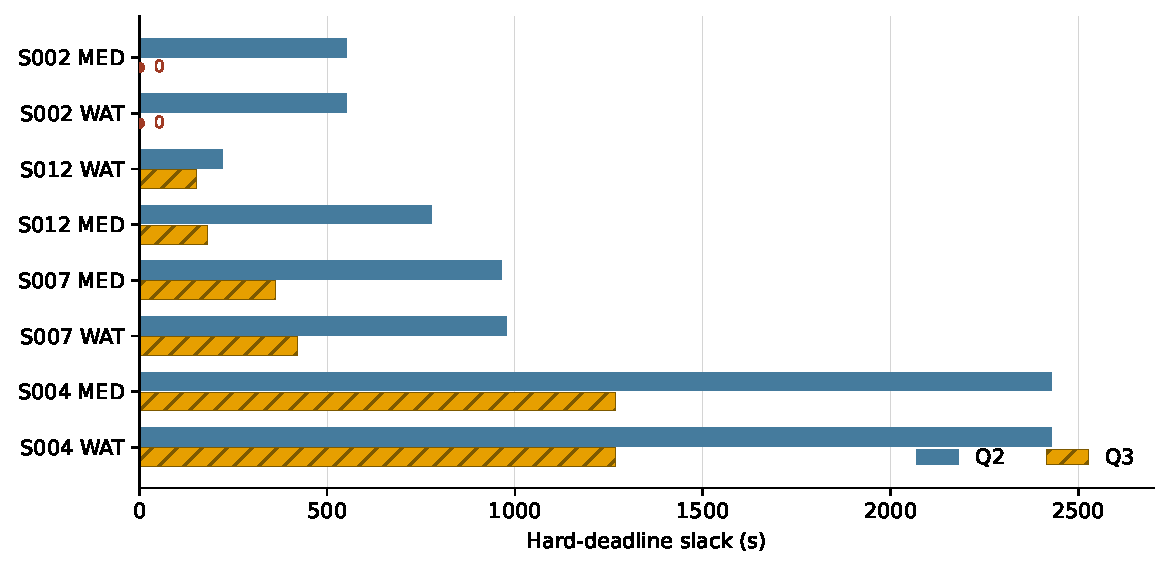
\includegraphics[width=0.8\textwidth]{figures/model_eval_hard_slack.pdf}
\caption{问题三余量最小的8个硬时限箱在问题二、三中的交付余量}
\label{fig:model-eval-hard-slack}
\end{figure}

图~\ref{fig:model-eval-link-margin}则按证明区间统计1317个保守链路裕量下界：其中127个区间低于1\,dB，最小为0.008976\,dB。图中的频数以\emph{区间个数}为单位，不以服务时长加权；它说明边界裕量不只由一个孤立采样点产生，但不能据此推断现场掉线概率或具体可容忍的定位误差。
\begin{figure}[htbp]
\centering
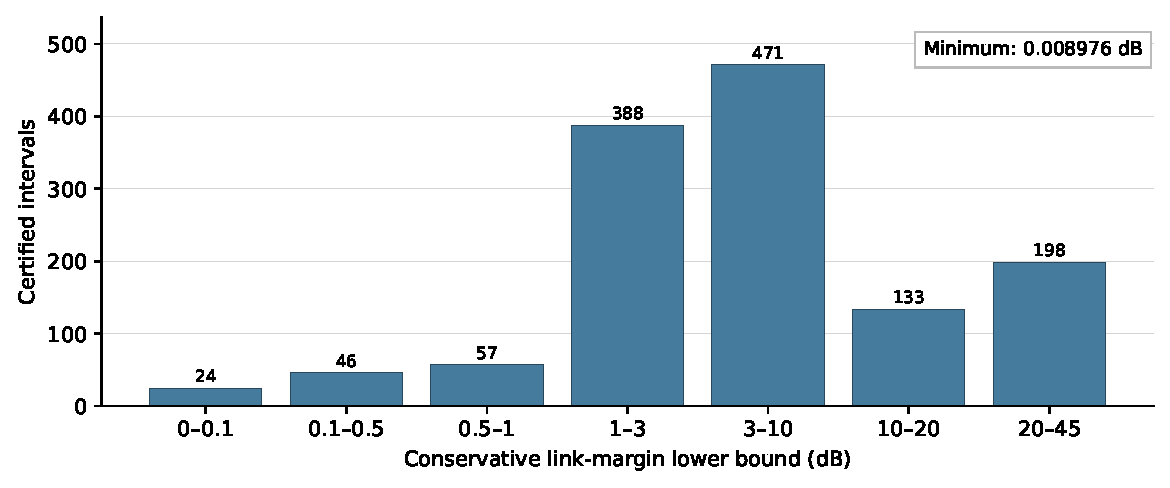
\includegraphics[width=0.8\textwidth]{figures/model_eval_link_margin.pdf}
\caption{连续通信证书的保守链路裕量下界分布}
\label{fig:model-eval-link-margin}
\end{figure}

进一步对同一正式方案作单因素保守敏感性检查：保持运输时刻、中继任务和证书选定的通信提供者不变，假设每条已用链路的路径损耗均额外增加$\Delta L$。若区间$I$原有的保守裕量下界满足$m_I-\Delta L\geq\varepsilon_L$，原区间证明仍成立；$\varepsilon_L$沿用连续证书的数值保护量。按区间时长加权，原证书可直接保留的需求时间比例为
\[
R(\Delta L)=\frac{\sum_{I:m_I-\Delta L\geq\varepsilon_L}|I|}{\sum_I|I|}.
\]
图~\ref{fig:model-eval-loss-stress}给出$0$--$5$\,dB附加损耗下的计算结果：增加1\,dB时，原证书仍覆盖90.4\%的需求时间；增加3\,dB时为61.3\%。由于最小裕量不足0.01\,dB，任何超过该值的统一附加损耗都使\emph{原证书}无法再覆盖全部时段。未保留证明的区间可能改由其他提供者保障，因此曲线既不是实际在线率，也不是重排任务后的最优覆盖率。
\begin{figure}[htbp]
\centering
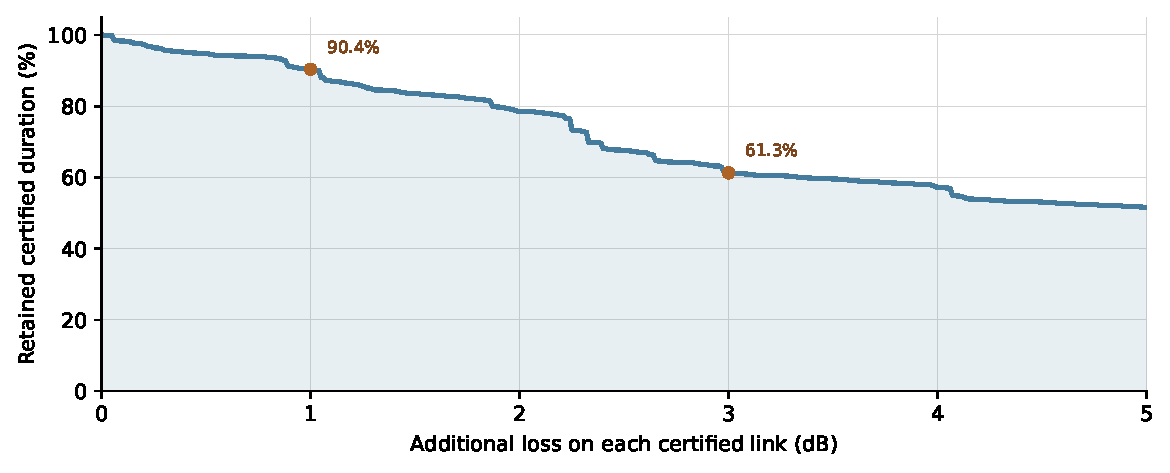
\includegraphics[width=0.80\textwidth]{figures/model_eval_loss_stress.pdf}
\caption{统一路径损耗后的原证书保留时长比例}
\label{fig:model-eval-loss-stress}
\end{figure}

\subsection{适用范围与结果复核}
本文的数值结论针对题给15个服务区、80个不可拆货箱、现有运输与中继设备、固定网关及所给DEM。运输路线、交付时刻和通信证书使用同一套地形与设备参数，但四问的输入依赖并不相同：问题一的安全载荷提供单架次物理边界，问题二选出的运输排程是问题三的起点，问题四又以问题三的正式任务和已选保障关系为固定基线。若服务区位置、设备性能、地形或通信参数发生变化，应从受影响的上游环节重新计算，不能直接沿用本题的24条运输路线、5条中继任务或三个不可拆分组。

结果复核也应遵循这一依赖次序。先用航段数据重算路线的载荷、飞行时间、能耗与返航电量，再核对逐箱交付和运输机、电池的占用区间；对第三问，还需检查中继机与组件占用、回传链路及连续证书是否覆盖全部运输通信需求，不能用离散采样记录替代区间证明；最后才根据证书中实际使用的中继关系重建第四问依赖图，并重新计算各组设备峰值。项目结果目录分别保存第二问的逐箱记录、第三问的正式解与连续证书、第四问的分区枚举结果，使每一级结论都能对应到原始计算记录。此复核链条检验的是模型内一致性，不等同于现场试飞或无线传播实测。

\subsection{局限与改进方向}
现有方案的边界主要有两点：问题二的候选路线与问题三的中继点、束搜索状态未穷尽全部可能，因此相应正式方案是经验证的可行解，不宣称全局最优；航时、能耗、充电和链路参数按题给值确定，图~\ref{fig:model-eval-hard-slack}和图~\ref{fig:model-eval-link-margin}所示的紧约束需要在实际部署前留出更充分的余量。这些边界不影响前述模型内可行性与第四问固定任务分区的穷尽性。

后续可先以最小硬时限余量和最小链路裕量为次级指标，联动细化运输时刻、中继服务窗及悬停位置，再用现有的逐箱、资源与连续通信证书重新验收。若需要更强的最优性结论，可按排程瓶颈扩充候选路线与中继点，并为路线选择及资源调度构造有效下界。若独立救援组优先于沿用问题三任务表，则可把组间隔离要求提前纳入联合调度。各项改进都能沿用本文的物理计算和分层验证框架，但新增性能应以重新求解后的结果报告。

\clearpage
%附录
\begin{appendices}
%\setcounter{page}{1} %如果需要可以自行重置页码。
\section{MATLAB 源程序}
\renewcommand{\thesubsection}{A\thinspace.\thinspace\arabic{subsection}}
\subsection{第1问程序}
\vspace{-2ex}

\begin{Matlab}{code.m}
clear all
kk=2;
[mdd,ndd]=size(dd);
while ~isempty(V)
    [tmpd,j]=min(W(i,V));
    tmpj=V(j);
    for k=2:ndd
        [tmp1,jj]=min(dd(1,k)+W(dd(2,k),V));
        tmp2=V(jj);
        tt(k-1,:)=[tmp1,tmp2,jj];
    end
    tmp=[tmpd,tmpj,j;tt];
    [tmp3,tmp4]=min(tmp(:,1));
    if tmp3==tmpd,
        ss(1:2,kk)=[i;tmp(tmp4,2)];
    else
        tmp5=find(ss(:,tmp4)~=0);
        tmp6=length(tmp5);
        if dd(2,tmp4)==ss(tmp6,tmp4)
            ss(1:tmp6+1,kk)=[ss(tmp5,tmp4);tmp(tmp4,2)];
        else, ss(1:3,kk)=[i;dd(2,tmp4);tmp(tmp4,2)];
        end
    end
    dd=[dd,[tmp3;tmp(tmp4,2)]];
    V(tmp(tmp4,3))=[];
    [mdd,ndd]=size(dd);kk=kk+1;
end;
S=ss; D=dd(1,:);
\end{Matlab}
\vspace{2ex}

\clearpage
\section{Python 源程序}
\renewcommand{\thesubsection}{B\thinspace.\thinspace\arabic{subsection}}
\subsection{第2问程序}
\vspace{-2ex}
\begin{Python}{mip1.py}
# This example formulates and solves the following simple MIP model:
#  maximize
#        x +   y + 2 z
#  subject to
#        x + 2 y + 3 z <= 4
#        x +   y       >= 1
#        x, y, z binary

# import gurobipy as gp
from gurobipy import * #GRB
try:
    # Create a new model
    m = Model("mip1")
    # Create variables
    x = m.addVar(vtype=GRB.BINARY, name="x")
    y = m.addVar(vtype=GRB.BINARY, name="y")
    z = m.addVar(vtype=GRB.BINARY, name="z")
    # Set objective
    m.setObjective(x + y + 2 * z, GRB.MAXIMIZE)
    # Add constraint: x + 2 y + 3 z <= 4
    m.addConstr(x + 2 * y + 3 * z <= 4, "c0")
    # Add constraint: x + y >= 1
    m.addConstr(x + y >= 1, "c1")
    # Optimize model
    m.optimize()
    for v in m.getVars():
        print('%s %g' % (v.varName, v.x))
    print('Obj: %g' % m.objVal)

except GurobiError as e:
    print('Error code ' + str(e.errno) + ': ' + str(e))

except AttributeError:
    print('Encountered an attribute error')
\end{Python}

\end{appendices}


\end{document}
